%% 
%% Copyright 2019-2020 Elsevier Ltd
%% 
%% This file is part of the 'CAS Bundle'.
%% --------------------------------------
%% 
%% It may be distributed under the conditions of the LaTeX Project Public
%% License, either version 1.2 of this license or (at your option) any
%% later version.  The latest version of this license is in
%%    http://www.latex-project.org/lppl.txt
%% and version 1.2 or later is part of all distributions of LaTeX
%% version 1999/12/01 or later.
%% 
%% The list of all files belonging to the 'CAS Bundle' is
%% given in the file `manifest.txt'.
%% 
%% Template article for cas-sc documentclass for 
%% double column output.

%\documentclass[a4paper,fleqn,longmktitle]{cas-sc}
\documentclass[a4paper,fleqn]{cas-sc}

% \usepackage[numbers]{natbib}
%\usepackage[authoryear]{natbib}
\usepackage[square,numbers]{natbib}
\usepackage{graphicx}
\usepackage{subcaption}
\usepackage{caption}
\usepackage{bm}
\usepackage{algorithmic}
\usepackage{hyperref}
 \usepackage[verbose]{placeins}
\DeclareCaptionLabelFormat{andtable}{#1~#2  \&  \tablename~\thetable}


\DeclareCaptionLabelFormat{twotable}{#1~#2  \&  \tablename~\the\numexpr\value{table}+1}
%%%Author definitions
\def\tsc#1{\csdef{#1}{\textsc{\lowercase{#1}}\xspace}}
\tsc{WGM}
\tsc{QE}
\tsc{EP}
\tsc{PMS}
\tsc{BEC}
\tsc{DE}
%%%

% Uncomment and use as if needed
%\newtheorem{theorem}{Theorem}
%\newtheorem{lemma}[theorem]{Lemma}
%\newdefinition{rmk}{Remark}
%\newproof{pf}{Proof}
%\newproof{pot}{Proof of Theorem \ref{thm}}

\begin{document}
\let\WriteBookmarks\relax
\def\floatpagepagefraction{1}
\def\textpagefraction{.001}

% Short title
\shorttitle{Graph neural networks for explainable EEG classification and prediction.}

% Short author
\shortauthors{Sz. Mazurek et~al.}

% Main title of the paper
\title [mode = title]{End-to-end automatic seizure detection in electroencephalography recordings using explainable graph attention networks }                      
% Title footnote mark
% eg: \tnotemark[1]
% \tnotemark[1,2]

% Title footnote 1.
% eg: \tnotetext[1]{Title footnote text}
% \tnotetext[<tnote number>]{<tnote text>} 
% \tnotetext[1]{This document is the results of the research
%    project funded by the National Science Foundation.}

% \tnotetext[2]{The second title footnote which is a longer text matter
%    to fill through the whole text width and overflow into
%    another line in the footnotes area of the first page.}


% First author
%
% Options: Use if required
% eg: \author[1,3]{Author Name}[type=editor,
%       style=chinese,
%       auid=000,
%       bioid=1,
%       prefix=Sir,
%       orcid=0000-0000-0000-0000,
%       facebook=<facebook id>,
%       twitter=<twitter id>,
%       linkedin=<linkedin id>,
%       gplus=<gplus id>]
\author[1,2]{Szymon Mazurek}[
                        auid=000,bioid=1,
                        orcid=0009-0006-7557-0157]

% Corresponding author indication
\cormark[1]

% Footnote of the first author
\fnmark[1]

% Email id of the first author
\ead{s.mazurek@sanoscience.org, szmazurek@agh.edu.pl}


%  Credit authorship
\credit{Conceptualization of this study, Methodology, Software, Data Curation, Validation, Visualization, Original draft writing and further editing}


\author[1,3]{Rosmary Blanco}[
    auid=001, bioid=2,
    orcid=0000-0002-5543-4557
]
\credit{Conceptualization of this study, Methodology, Data Curation, Investigation, Formal Analysis, Review and editing}

\author[1,2,3]{Joan Falc\'o-Roget}[
    auid=002, bioid=3,
    orcid=0000-0002-9410-6361
]
\credit{Conceptualization of this study, Methodology, Software, Visualization, Validation, Original draft writing and further editing}

\author[1,2]{Alessandro Crimi}[
    auid=003, bioid=4,
    orcid=0000-0001-5397-6363
   ]
\credit{Conceptualization of this study, Methodology, Validation, Supervision, Project administration, Resources, Review and editing}



\affiliation[1]{organization={Sano Centre for Computational Medicine},
    addressline={Czarnowiejska 36}, 
    city={Cracow},
    postcode={30-054 Cracow}, 
    country={Poland}}
    
\affiliation[2]{organization={AGH University of Science and Technology},
    addressline={Adam Mickiewicz Avenue 30}, 
    city={Cracow},
    postcode={30-059 Cracow}, 
    country={Poland}}
    
\affiliation[3]{These authors contributed equally to this work}

% Corresponding author text
\cortext[cor1]{Corresponding author}

% Footnote text
% \fntext[fn1]{This is the first author footnote. but is common to third
%   author as well.}
% \fntext[fn2]{Another author footnote, this is a very long footnote and
%   it should be a really long footnote. But this footnote is not yet
%   sufficiently long enough to make two lines of footnote text.}

% For a title note without a number/mark
% \nonumnote{This note has no numbers. In this work we demonstrate $a_b$
%   the formation Y\_1 of a new type of polariton on the interface
%   between a cuprous oxide slab and a polystyrene micro-sphere placed
%   on the slab.
%   }

% Here goes the abstract
\begin{abstract}
Epilepsy, the most common neurological disorder worldwide caused by abnormal electrical activity in the brain, represents a great challenge for modern healthcare. The disorder manifests itself by recurrent periods of hyper-synchronized brain activity, or seizures, greatly hampering the quality of an affected person. Proper diagnosis and monitoring of the disease are crucial for the therapy outcomes. Electroencephalography, the most common measurement technique in epilepsy, allows for recording the patient's brain activity via scalp potentials. However, accurate analyses are time-consuming and require a trained expert's knowledge. In this paper, we exploit the non-euclidean relationships between electrodes using graph neural networks. We build our solution using a end-to-end approach, starting with determining optimal pre-processing and class balancing techniques, performing neural architecture search, and using existing algorithms to create explanations for the model's predictions. Our model achieves high performance of 0.9786 AUROC and 92.11 \% balanced accuracy in the final, 10-fold cross-validation evaluation, comparable with the existing state-of-the-art solutions, while also showing promising results in predicting the seizure onset. Obtained explanations provide insights about feature importance and changes in functional connectivity, being consistent with the current clinical knowledge. We also show that the network reliably classifies preictal activity up to 1 hour before seizure occurrence, opening a way to be used as a seizure predictor.
\end{abstract}

% Use if graphical abstract is present
% \begin{graphicalabstract}
% \includegraphics{figs/grabs.pdf}
% \end{graphicalabstract}

% Research highlights
\begin{highlights}
\item We research EEG pre-processing and class balancing methods, concluding that it impacts the AI model’s performance
\item Bayesian architecture search is used to quickly configure the network's hyperparameters for robust performance
\item Algorithms for explaining graph neural network predictions are used to determine both relevant features and changes in brain connectivity
\item Model for EEG time window classification can also be used as a robust seizure predictor 
\end{highlights}

% Keywords
% Each keyword is seperated by \sep
\begin{keywords}
epilepsy \sep electroencephalography \sep seizure detection \sep seizure prediction \sep graph neural networks  \sep explainable AI
\end{keywords}

\maketitle

\section{Introduction}
Epilepsy, a neurological disorder characterized by recurrent seizures stemming from abnormal electrical activity in the brain, ranks as the fourth most prevalent neurological condition globally, impacting an estimated 50 to 60 million individuals worldwide \cite{PeruccaEpilepsyWorldwide,ThurmanEpilepsyWorldwide}. Electroencephalography (EEG) serves as a pivotal tool in the diagnosis of epilepsy, playing a central role in defining the epileptogenic cortex and identifying abnormal brain activity associated with seizures. Additionally, EEG is useful in pinpointing the source region of epilepsy, facilitating the planning of surgical interventions \cite{JehiEpilepticZone}. Recent years have witnessed notable advancements in EEG technology, enhancing its accuracy and reliability in both the diagnosis and treatment of epilepsy. However, the correct identification of seizure-related periods remains a challenging task for practitioners, as well as the prediction of future seizures.

Concurrently, the past decade has witnessed substantial advancements in the field of artificial intelligence (AI), with medicine emerging as a major beneficiary of its transformative capabilities. AI algorithms, adept at detecting subtle patterns and anomalies in medical data, are expected to play a crucial role in improving diagnostic accuracy and, consequently, enhancing patient outcomes. Furthermore, if successfully deployed, these technologies can enhance specific clinical processes, such as minimizing the time required for diagnostics. These and other advancements have significantly influenced the domain of computer-aided seizure analysis, with deep learning emerging as the predominant research approach from the algorithmic perspective. 

\subsection{Deep learning algorithms for EEG classification}

% Add a section describing other approaches RNNs, CNNs, etc.
To solve the EEG classification problem, various deep-learning approaches can be used. They exploit information in the time domain, frequency domain, and time-frequency domain. For example, Wang et. al. used the time domain features via a 1D convolutional neural network (CNN) to classify epileptic EEG periods \cite{Wang1DCNNPrediction}. Yao et. al. created an attention-based long-short term memory (LSTM) architecture to analyze temporal properties of the signals \cite{YaoBiLSTM}. Li and Chen worked in the frequency domain, applying the fast Fourier transform (FFT) to the signal before using a CNN-based architecture to perform classification \cite{LiChenFFTCNN}. Additionally, combining spectral and temporal features has been shown to result in improved results \cite{AssaliTemporalSpectralCNN, GaoWaveletCnnClassification}.

Recently, graph neural networks (GNNs) have also been used extensively in EEG classification. The choice of this kind of neural network poses a significant advantage compared to the previously described algorithms, as they allow to conveniently model non-Euclidean relationships in the data \cite{BronsteinGeometricDL}. These kinds of relationships are ubiquitous in the real world, and also in the human brain, which is a massively complex network. EEG data easily fits this view, where the electrodes and their mutual relationship can be viewed in the form of a non-Euclidean structure, therefore allowing to model it with a graph.
Zhao et.al. use  GNN and focal loss \cite{lin2020focal} to discriminate between seizure and non-seizure samples in the frequency domain \cite{ZhaoGraphFocalLoss}. 
Graph isomorphism network is used by Tao et.al. \cite{tao2022gnnisomorphism} to exploit brain connectivity and perform the detection. Jibon et. al. combine the usage of GCN with CNN to perform ensemble prediction exploiting spectrotemporal information\cite{jibon2023gcndnn}.
Attention-based GNNs have also been employed for this task with success \cite{zhao2021seizuregat}. He et. al. extends 
 the usage of GAT by also incorporating LSTM to automatically extract time domain relationships from the analyzed signals \cite{he2022gatblstm}.
Lastly, seizure prediction was also widely explored by proposing a simple GNN to efficiently detect preictal periods in the signals \cite{JiaEfficientGraphConv}. 

Noteworthy, operating on graph structures allows one to conveniently obtain explainability measures for models' decisions. In recent work, Raeisi et. al. use learned edge attention coefficients in GAT to highlight changes in brain connectivity when performing EEG classification \cite{raeisi2023explainable}. Explainability is especially important for medical applications, where trustworthiness is a key factor in deciding on the adoption of computer-aided diagnosis systems.


% Before delving into the proposed framework, let's review some current controversies related to EEG analysis. 

\subsection{Existing methodological heterogeneities}

The realm of solutions mentioned above is characterized by significant heterogeneity. These solutions exhibit variations not only in their employed algorithms but also in their approaches to pre-processing, handling class imbalances, and evaluating the results.
\subsubsection{EEG pre-processing}

EEG signals are raw brainwave recordings with small amplitudes (in the order of $\mu$V) and frequencies up to 300 Hz. However, they suffer from contamination by various interferences, including artifacts from the measurement system, environmental sources (e.g., like power line noise or electromagnetic fields), and other biological signals unrelated to brain activity (e.g., electrooculogram, electromyogram, electrocardiogram). These artifacts can severely degrade the signal quality, thus necessitating an increase in the signal-to-noise ratio to preserve the valuable information. To achieve this, standard pre-processing steps ought to be employed, including filtering, re-referencing, interpolating bad channels, and removing artifacts through various methods such as signal decomposition, wavelet filtering, template subtraction, and regression \cite{kim2018preprocessing}. These steps help in cleaning the EEG data and ensuring the accurate interpretation of brain activity.

The selection of artifact elimination techniques depends on the nature of the analyzed data and the subsequent analysis. However, eliminating artifacts in EEG remains a challenging task, often requiring manual intervention and expert domain knowledge. This process is time-consuming and may introduce errors due to its subjective nature. To address these challenges, researchers have sought to formalize and automate EEG denoising, leading to various studies in the literature \cite{GeethaEEGDenoise,UpadhyayEEGDenoise,SatyenderEEGDenoise,MumtazEEGArtifactReview}.
Among the blind source separation-based methods commonly used for cleaning EEG signals, principal component analysis (PCA) \cite{ShlensPCA} and independent component analysis (ICA) \cite{HyvarinenICA} stand out. ICA has shown promising results, especially for removing blinks and muscular artifacts. However, it often requires expert visual inspection of all components to discard those related to artifacts, making it a time-consuming process, even with the aid of automatic artifact recognition algorithms \cite{LiIcalabel}. On the other hand, the PCA method has demonstrated faster and less computationally demanding performance, providing effective results for both dimensionality reduction and artifact elimination \cite{MumtazEEGArtifactReview}.

Research has demonstrated that EEG artifact removal methods can enhance the readability of EEG signals for various tasks, benefiting both human experts and automated algorithms \cite{JinArtifactSota, KunjiraPreprocessingEEG}. Therefore, this stage is crucial when applying deep learning methodologies for seizure detection. Within the literature, there is considerable diversity in the pre-processing steps undertaken prior to EEG signal classification. Some authors employ basic techniques like band-pass \cite{JiaEfficientGraphConv} or wavelet \cite{GaoWaveletCnnClassification} filtering, while others opt for more advanced decomposition and filtering methods \cite{GiudiceCNNAdvancedPrepro}. Some even work with raw, unprocessed data without applying any pre-processing technique \cite{LiChenFFTCNN, Wang1DCNNPrediction, YaoBiLSTM}.

\subsubsection{Class imbalance handling}
Another problem arising naturally when performing EEG classification with automated methods is the class imbalance problem. EEG signals typically consist of extended recordings where epileptic seizures are relatively rare events. Therefore, ictal activity is naturally unbalanced w.r.t. non-pathological brain activity. Therefore, class balancing is not only recommended but often necessary \cite{abd2013imbalance}.
In the literature, similarly to the pre-processing, this problem is also handled diversely by the researchers. Utilized methods encompass undersampling, where the majority class samples are reduced to match the number of minority class samples, oversampling, which involves duplicating minority class samples to balance the data \cite{JiaEfficientGraphConv}, and modifications to the loss function \cite{ZhaoGraphFocalLoss}. Additionally, using time windows that overlap during sample extraction is another approach employed to address the issue of class imbalance \cite{ZhaoGraphFocalLoss,he2022gatblstm}. A growing body of literature also shows promise by using deep generative models to artificially generate more data samples in minority classes \cite{chao2021GanAug}.




% Additionally, the comparability of results remains a concern, as different studies often utilize distinct performance metrics. Moreover, the methods for partitioning the data vary, with some researchers employing classic k-fold cross-validation \cite{tao2022gnnisomorphism}, while others prefer leave-one-out cross-validation and its modifications \cite{JiaEfficientGraphConv, ZhaoGraphFocalLoss}. Finally, certain studies choose to use only a subset of patients or recordings, excluding outlier cases, which could potentially limit the real-world applicability of their findings \cite{JiaEfficientGraphConv, wang2023plvgraphs}.

\subsection{The aim of the study}
Taking into consideration those aspects, 
in this paper, we aimed to create an end-to-end approach for creating models handling the problem of EEG classification in epileptic patients using graph neural networks. We start with the evaluation of the often neglected, but crucial step of proper data pre-processing and handling of the class imbalance inherently present in EEG datasets. Then, building on that, we perform a neural architecture search using the Bayesian approach to obtain the model's architecture and hyperparameters that lead to the best classification performance. We then evaluate the obtained model and compute explanations that show the changes in feature and edge relevance between predictions for different classes. Finally, we evaluate the usefulness of the trained classifier as an indirect seizure event predictor, showing its ability to maintain accuracy even with increasing predictive horizon.  The workflow can be seen in the Figure \ref{fig:graphical-abstract}.
The code and instructions for reproducing the results are available at \url{https://github.com/szmazurek/sano_eeg}.

\begin{figure}[!h]
    \centering
    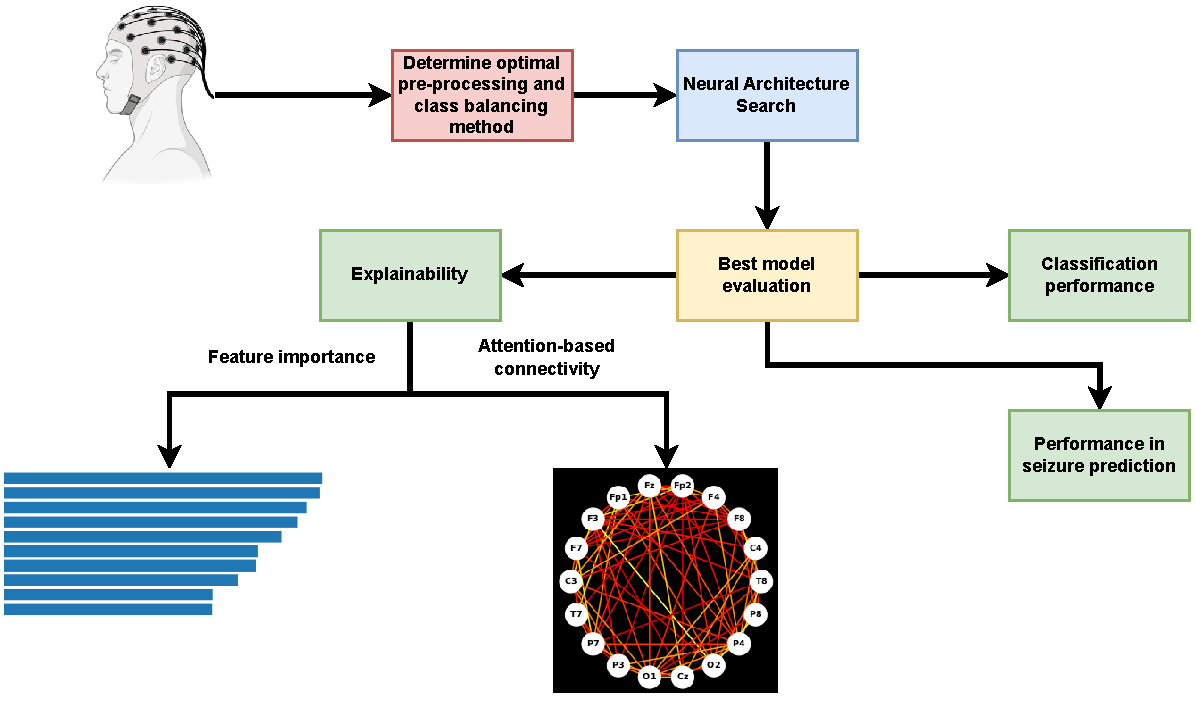
\includegraphics[scale=0.8]{figures/graphical_abstract.pdf}
    \caption{The proposed workflow: First, we represent EEG recording signals as a graphs. Next, optimal pre-processing and class balancing method is established. This knowledge is then incorporated in neural architecture search procedure, which automatically find the best performing model. Finally, extensive evaluation of the found model is performed -  we compute performance metrics, explainability scores and evaluate the model's usefulness in seizure prediction task.}
    \label{fig:graphical-abstract}
\end{figure}

\section{Materials and methods}

\subsection{Dataset}
Details regarding the data are thoroughly described in the Children's Hospital Boston (CHB-MIT) repository \cite{ShoebChbmit}. Data contained 916 hours of EEG recordings from 23 patients between 1.5 and 22 years of age. One subject was scanned a second time after 1.5 years but the samples were treated as independent (i.e., a total of 24 recordings). All patients exhibited drug-resistant epilepsy and had not taken medication prior to the recordings. A total of 23 to 26 electrodes with a sampling rate of 256 Hz and 16-bit resolution were placed following the international 10-20 system. Altogether, 198 seizures were annotated by clinical experts after discarding epileptic activity shorter than 6 seconds. Despite its potential impact on the model's performance, more detailed annotation would require extensive work from experts. 

% \subsection{Graph neural networks}

\subsection{Graph neural networks and attention mechanism}
GNNs can learn non-trivial representations by leveraging the complex topological organization of the data \cite{velivckovic2023everything,wu2019graphsurvey}. Intuitively, a graph constitutes a non-Euclidean geometric space where complex relationships between data points can be embedded and forwarded as inputs into a GNN \cite{BronsteinGeometricDL}. More formally, a graph $\mathcal{G} = (\mathcal{V}, \mathcal{E})$ is defined as a set of nodes $\mathcal{V} = \{1, \ldots, n\}$ and a set of edges $\mathcal{E} = \{(i,j) \ | \  i,j \in \mathcal{V}\}$ where $(i,j)$ represents a link or interaction between the $i$-th and $j$-th nodes. Initially, each node $i \in \mathcal{V}$ is associated with a column feature vector $\mathbf{h}_{i}^{(0)} \in \mathbb{R}^{d^{(0)}}$.

Every layer $l$ of a GNN updates the hidden representation of each node by aggregating information from the neighborhoods: 
\begin{equation} \label{layer}
    \mathbf{h}_{i}^{(l+1)} = f_{\theta} \left( \mathbf{h}_i^{(l)}, \textsc{F} \left( \{ \mathbf{h}^{(l)}_j \, | \, j \in \mathcal{N}_i \} \right) \right),
\end{equation}
where $\textbf{h}_{i}^{(l+1)} \in \mathbb{R}^{d^{(l+1)}}$ are the new node representations, $\mathcal{N}_i$ is the neighborhood of the $i$-th node, $f_{\theta}$ denotes a nonlinearity, and $\textsc{F}$ is a permutation-invariant aggregator. Several proposals exist for the aggregation operator, determining the expressive power, interpretability, learning stability, and scalability of the network \cite{velivckovic2023everything}. Attentional aggregators offer an interesting trade-off by independently aggregating local information and subsequently scoring the relevance of each edge for the final prediction \cite{velickovic2018graph}. Following \cite{brody2021gatv2}, we computed a scalar score,

\begin{equation} \label{score_e}
    e_{i,j}^{(l)} = \mathbf{a}^{(l)\top}  \cdot \textsc{LeakyReLU}(\mathbf{W}^{(l)} \cdot [\mathbf{h}_{i}^{(l)} || \mathbf{h}_{j}^{(l)}]),
\end{equation} 

where $\mathbf{a}^{(l)} \in \mathbb{R}^{d^{(l+1)}}$ and $\mathbf{W}^{(l)} \in \mathbb{R}^{d^{(l+1)} \times 2d^{(l)}}$ are learned parameters, and $||$ concatenates $\mathbf{h}_{i}^{(l)}$ and $\mathbf{h}_{j}^{(l)}$ along the first axis. These scores are normalized within the neighbors,

\begin{equation} \label{score_alpha}
    \alpha_{ij}^{(l)} = \frac{\exp\left(e_{ij}^{(l)}\right)}{\sum_{k \in N_i\cup\{i\}} \exp\left(e_{ik}^{(l)}\right)},
\end{equation}

where $\alpha_{ij}^{(l)}$ is the final attention score of each edge. Lastly, we computed the new representations learned by the $l$-th layer by weighting the features with the learned attention scores: 

\begin{equation} \label{representation}
    \textbf{h}_{i}^{(l+1)} = f_{\theta}\left( \sum\nolimits_{j \in N_i \cup\{i\}} \alpha_{ij}^{(l)} \mathbf{W}^{(l)} \cdot \mathbf{h}_{j}^{(l)} \right).
\end{equation}
In practice, multiple attention \textit{heads} have been proven to improve the stability of learning \cite{velickovic2018graph,brody2021gatv2}. For each head, an independent attention score $\bm{\alpha}_n^{(l)}$ is learned (i.e., in Eq. (\ref{score_alpha})). Finally, the outputs in Eq. (\ref{representation}) of all $N_K^{(l)}$ heads are concatenated or averaged to give the $l+1$ layer node representation.

\subsection{Neural architecture search}

Neural architecture search (NAS) is a process of automatically finding the optimal architecture of a neural network to solve a given problem. The architecture of the network can be viewed as a composition of various layers of neurons, connections between them, and hyperparameters defining their properties. 
Formally, NAS can be defined as finding an architecture in a search space within the computation budget, which will be able to achieve the best performance, as measured by a chosen metric for a given training dataset \cite{white2023neural}. To this day, various NAS approaches have been introduced, aiming mostly to narrow the search space or increase the effectiveness of searching through it. To name a few, popular solutions are based on evolutionary algorithms, reinforcement learning, Monte Carlo trees, or Bayesian optimization \cite{white2023neural}. 
Formally, Bayesian architecture search consists of using the surrogate model to obtain the approximation of the chosen objective function we aim to optimize.
This surrogate model is simply an estimation of posterior probability using Bayes theorem,
\begin{equation} \label{NAS_surrogate}
    P(m|a) =  \frac{P(a|m)P(m)}{P(a)}
\end{equation}
where $a \in A$ is an architecture configuration chosen. The evidence, namely the metric score $m$ evaluates the performance of the neural network trained with the chosen architecture $a$. 
This model is then used to guide the search by choosing the next $a'$ for evaluation. In this paper, candidate architectures are chosen based on the
expected improvement (decrease) of the mean cross-entropy value across test folds (see section \ref{section:experiment_desing}). First, let us denote the improvement value for a given hyperparameter combination $I(a)$ for the minimization problem as:
\begin{equation}
    I(a) = \text{min }(f(a) - f(a^{best}),0) = \text{min }(m - m^{best},0),
\end{equation}
$f$ is a function evaluating the given $a$, $a^{best}$ is the best architecture found so far (leading to the smallest value of $f$, namely $m^{best}$).
Therefore, we can define the \textit{expected improvement} as:
\begin{equation}
    EI(a) = \mathbb{E}[I(a)] = \int_{-\infty}^{m_{best}}|I(a)|P(m|a)dm.
\end{equation}
The architecture $a$ that maximizes $EI(a)$ is the next point to be evaluated by the surrogate model in Eq. \ref{NAS_surrogate}, which is then updated following a Gaussian process. Thus, with every iteration, the algorithm determines more optimal architectures by effectively balancing exploration and exploitation \cite{elsken2019neural,white2023neural}. 

%write an expected improvement equation here. Determine what is threshold and how is it chosen in wandb (the threshold is the minimal or maximal value obtained in the metrics so far. Note that depending on the task (minimization or maximalization, we evaluate the behaviour of expected improvement differently


\subsection{Explainable seizure detection with GNNs}
As outlined earlier in the introduction, we aimed to explain the network's focus when detecting the presence of an epileptic seizure. We restricted our attempts to provide intuitive explanations of the most important edges and features.

Edge importance can be directly assessed by averaging the attention scores in Eq. (\ref{score_alpha}) overall $N_K^{(l)}$ attention heads in a given layer 

\begin{equation} \label{edge_explain}
    \mathbf{A}^{(l)} = \frac{1}{N_K^{(l)}} \sum_{n=1}^{N_K}  \bm{\alpha}_{n}^{(l)}.
\end{equation}

On the other hand, feature importance aims to identify a subgraph $\mathcal{G}_{S} \in \mathcal{G}$ and associated features $\mathcal{H}_{S} = \{ \mathbf{h}_i \mid i \in \mathcal{V}_{S} \}$ relevant for the GNN predictions \cite{Ying2019GnnX}. A separate \textit{explainer} model is optimized to maximize the mutual information $MI$ between the predicted labels $Y$ and the selected subgraph and features $(\mathcal{G}_S,\mathcal{H}_S)$: 

\begin{equation}\label{mutual_info}
    \max_{\mathcal{G}_{S}, \mathcal{F}} MI(Y, (\mathcal{G}_{S}, \mathcal{F})) = H(Y) - H(Y \mid \mathcal{G}_{S}, \mathcal{H}_{S}^\mathcal{F}),
\end{equation}
where $H(\cdot)$ is the Shannon entropy, $\mathcal{H}_{S}^\mathcal{F} = \mathcal{H}_{S} \odot \mathcal{F}$ is a subset of masked features, and $\mathcal{F}$ is a learned binary mask identifying the most informative features of the selected subgraph.
The feature explainability scores $\mathcal{F}$ were obtained for every sample and later averaged for every class. 

\subsection{Signal pre-processing}
We first unified the electrode montages across the recordings. We chose 18 channels that are present in all of them. The final layout can be seen in Fig. \ref{fig:ch-layout}.
% namely FP1-F7, F7-T7, T7-P7, P7-O1, FP1-F3, F3-C3, C3-P3, P3-O1, FZ-CZ, CZ-PZ, FP2-F4, F4-C4, C4-P4, P4-O2, FP2-F8, F8-T8, T8-P8 and P8-O2. 
During initial trials, we employed PrepPipeline \cite{BigdelyPrep_pipeline} and ICA decomposition coupled with an automated component labeling algorithm \cite{LiIcalabel} as the primary method to remove artifacts from the signal. Unfortunately, the results were unsatisfactory, as the amount of noise and bad channels led to the failure of the methods on most of the recordings.
Subsequently, we devised an alternative method by combining a filtering process, re-referencing, and PCA decomposition for artifact removal. 
The goal was to effectively remove prevalent eye blinks, muscular artifacts, and power line noise from the EEG data. In EEG signals, variance represents the level of fluctuation in the recorded electrical activity from the scalp. Artifacts can significantly contribute to the overall variance, particularly when they possess large amplitudes and occur frequently, as seen with eye blinks and muscle activity. Thus, the variance explained by each component after the PCA decomposition can serve as a useful indicator of artifact presence in the data. Moreover, the orthogonality preservation of the components in this method enables the automatic selection of those representing artifact-related activity. However, it is crucial to note that not all artifacts exhibit high variance. For instance, certain types of environmental noise, like electrical interference from power lines at 50 Hz, may have low amplitudes and contribute relatively little to the overall variance of the signal, yet they can be easily addressed and eliminated through proper band-pass filtering.
\begin{figure}[b]
    \centering
    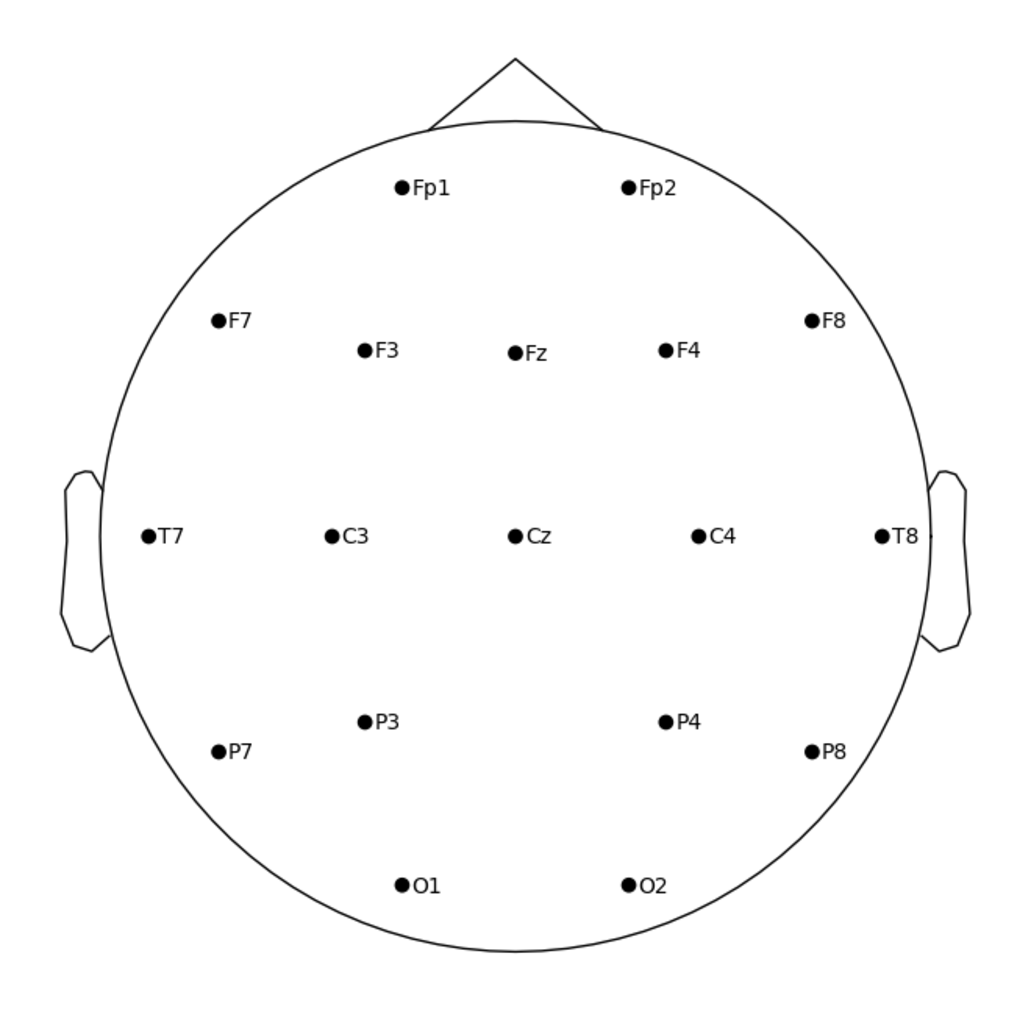
\includegraphics[scale=0.4]{figures/electrodes.pdf}
    \caption{Layout of the electrodes used during the experiments.}
    \label{fig:ch-layout}
\end{figure}

The proposed pipeline involves the following steps: first, recordings undergo a filtering procedure, limiting the frequencies to a range between 0.5 and 30 Hz. This selection aims to preserve the EEG frequency content relevant to the resting-state condition. Subsequently, the channels are average-referenced, and finally, PCA is applied to effectively eliminate any remaining significant artifacts present in the signals by discarding the first two principal components. The procedure is summarized in Figure \ref{fig:proposed-filtering}.

\begin{figure*}
    \centering
    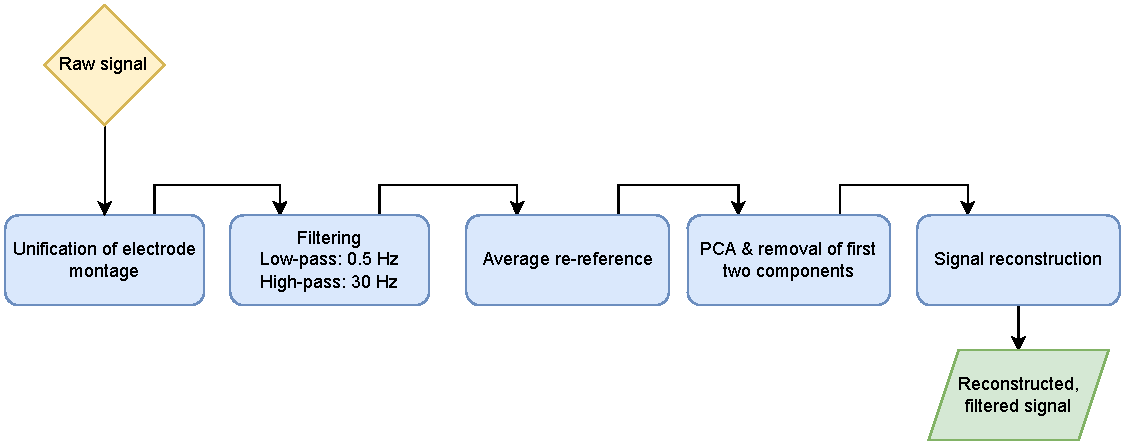
\includegraphics[scale=0.8]{figures/prepro-steps.pdf}
    \caption{Visualization of the proposed pre-processing method for EEG data.}
    \label{fig:proposed-filtering}
\end{figure*}

\subsection{Class imbalance handling methods}
To assess the impact of class imbalance handling, we evaluated commonly used techniques from the machine learning domain. For this study, the following methods have been chosen for evaluation:

\textit{Undersampling}, a technique to discard random samples from the majority class until the demanded ratio between classes is obtained.

\textit{Class weighting}, a modification to the loss function, where errors on chosen classes, usually minority ones, are weighted such that the model receives a higher penalty for erroneous predictions on these.

\textit{Overlap during time window extraction}, leading to an increased number of samples for classes that the overlap was assigned to.

\textit{SMOTE (Synthetic Minority Oversampling Technique) \cite{ChawlaSMOTE}}, a classic algorithm that is able to create new, plausible artificial samples for minority classes.

\subsection{Sample extraction}

Time windows used for training and evaluating the models were chosen based on the mentioned earlier minimal length of abnormal activity determining the seizure, namely 6 seconds. The classes were determined in the following way: ictal periods were determined using human annotations provided in the dataset. The preictal activity was defined within the 10 minutes before seizure onset. Additional 15-second buffer periods before and after seizures were discarded. This decision was based on the possible presence of pathological activity during these periods, which, while not explicitly labeled as seizures by the clinician, exhibited characteristics that warranted exclusion to ensure the purity of the seizure-specific data. Interictal periods were extracted from the recordings of a given patient that did not contain seizure activity, starting from the randomly chosen time point. Noteworthy, the number of interictal samples extracted were matching the number of preictal ones for a given subject. This step was taken to prevent further class imbalance, which was already significant due to the small number of ictal samples. Initially, the imbalance ratio was roughly 1:8 for ictal to preictal for every patient.

\subsection{Experimental design}
\label{section:experiment_desing}
%In this study, we used a step-by-step approach, building on the consecutive experiments based on the findings from the previous ones. We also note that pre-processing part of this study was also extensively described in our previous work \cite{mazurek2023preprocessing}.
The ultimate goal of this study was to develop a thorough end-to-end deep learning-based seizure detection workflow. To do so, we conducted a set of sequential experiments starting from the evaluation of different pre-processing and class-imbalance approaches \cite{mazurek2023preprocessing}, followed by accurate GAT-based architecture searches, EEG network reconstruction, explainable AI predictions, and an evaluation of the final model's predictive horizon. In what follows, we provide a detailed account of each step of the process.

\subsubsection{Evaluating pre-processing and class balancing methods}
To evaluate the impact of artifact and imbalance removal, we devised a simple experiment, where we aimed to detach the differences in the model's performance from both the graph construction approach and model design. We therefore did not implement any techniques for specific modifications of graph adjacency matrices. A complete graph $\mathcal{G}_{sw} = (\mathcal{V}_{sw},\mathcal{E}_{sw})$ was created for each subject $s$ and time window $w$, with $\mathcal{V}_{sw} = \{i \ | \ i=1,\ldots,18\}$ and $\mathcal{E}_{sw} = \{(i,j)_{sw} \ | \ i,j \in \mathcal{V}_{sw}\}$. Each node $\mathcal{n}_{sw} \in V_{sw}$ represented a single EEG electrode and was associated with feature vector $\mathcal{x_{sw}}$, with the corresponding time series data. 

For these experiments, the problem was reduced to a binary classification between ictal and preictal samples to further simplify the approach and shorten the time required to conduct subsequent training procedures. We therefore looked to minimize the binary cross entropy loss using optimizer AdamW \cite{LoshchilovAdam} with a learning rate of $10^{-4}$ and a weight decay of $10^{-3}$. As a performance metric, we chose the Area Under the Receiver Operating Characteristic (AUROC), as it provides information about the model's ability to separate between classes without the need to tune the threshold value necessary in most popular metrics. Also, in contrast to accuracy, it does not provide deceptively high scores in imbalanced learning scenarios \cite{fawcett2006roc}. 

The model was evaluated using Leave-One-Out Cross-Validation (LOOCV), where one subject was excluded from the data for testing purposes. The training set was further split to obtain a validation subset, consisting of 10\% of the remaining training data. This split was performed with stratification on both classes and subjects to ensure that the class ratio and number of samples from a given patient in both sets were approximately equal.

Finally, we performed additional processing on the time series $x_{sw}$. We z-score standardized the samples, using all the samples except the ones left for testing for a given training run to extract the mean and standard deviation. Testing data was standardized with the same statistics. Finally, we extracted the power spectrum using a fast Fourier transform. This step allowed us to use the GATv2 layer straightforwardly, without the need to incorporate handling of temporal relationships in the layer.
We constructed a simple graph neural network, adhering to the common practices without any extensive architecture or hyperparameter tuning. The initial architecture can be seen in Fig. \ref{fig:initial-network}.

\begin{figure}[h]
    \centering
    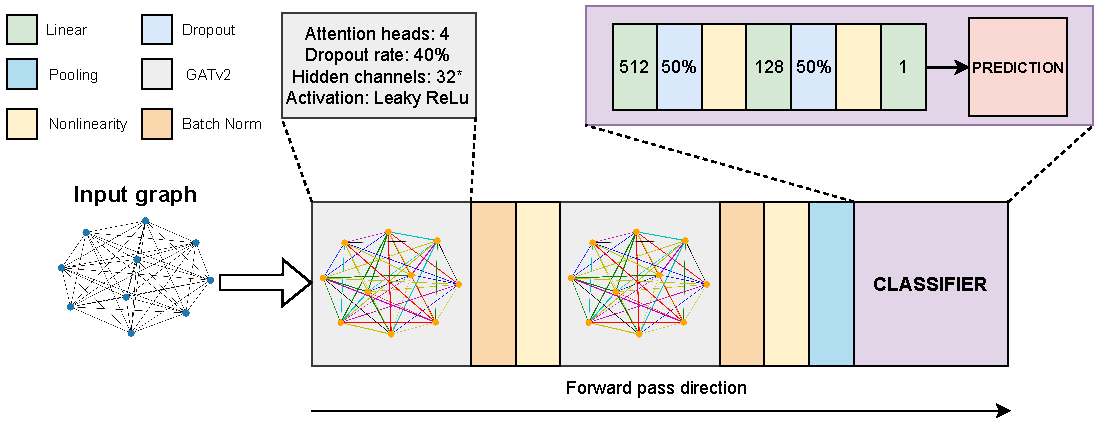
\includegraphics[scale=0.85]{figures/network_initial_elsvier.pdf}
    \caption{The graph presenting initial network architecture. Numbers in the blocks denote the number of neurons and probability for fully-connected and dropout layers respectively. In this experiment, the nonlinearity used was Leaky ReLu. \newline
    * The number of hidden channels in the second GATv2 layer was set to 64. 
    }
    \label{fig:initial-network}
\end{figure}

\subsubsection{Neural architecture search}

For the NAS procedure, we incorporated the findings from the previous experiments. We used the proposed pre-processing approach to remove the artifacts from the data. The classification problem was extended to multiclass classification, by introducing previously discarded interictal class. Samples were created with the 5-second overlap. The loss function, cross-entropy, was minimized with the usage of class weights proportional to the share of a given class in the entire dataset. The weights were obtained using the following formula \cite{king2001regression}:
\begin{equation}
    Cw_{i} = \frac{n_{s}}{n_{c}n_{s}^{i}},
\end{equation}
where $Cw_{i}$ is the weight of class $i$, $n_{s}$ is the number of samples in the dataset, $n_{c}$ is the number of unique classes in the dataset and $n_{s}^{i}$ is the number of samples representing class $i$.
During the visual inspection of the pre-processed data, some artefactual activity was still present, manifesting mostly in periods of supra-physiological amplitude peaks of varying lengths. Due to this fact, we decided to standardize the data using robust standard scaling instead of classic z-score normalization. This approach allows one to properly standardize the data containing outliers by using the median instead of the mean and interquartile range between 75-th and 25-th percentile instead of standard deviation. These parameters were extracted from the interictal period instead of the preictal one as one is a better description of the baseline.

At this stage, we decided to incorporate a more sophisticated algorithm for creating connections between edges in the graphs representing the samples. There is evidence suggesting that explicitly defining edges instead of creating a complete graph can enhance the performance of graph neural networks (GNNs) for this specific problem. Particularly, research studies have shown that utilizing connectivity measures between EEG channels in the samples leads to improved results compared to using geodesic distance between electrodes.

In the work by Wang et. al. \cite{wang2023plvgraphs}, authors demonstrate that computing the Phase Locking Value (PLV) \cite{bruna2018plv} for each sample and creating an edge between the nodes if the corresponding value is above the threshold improves the performance compared to using geodesic distance and spectral correlation-based connectivity. The threshold is set as the mean value of PLVs for a given sample. Formally, the adjacency matrix creation can be expressed by the Equation \ref{edges} and \ref{threshold}.

\begin{equation}
    (i,j)_{sw} =  
    \begin{cases}
        1 \text{  if  PLV}(r_{swi}(t), r_{swj}(t)) > \epsilon_{sw} \\
        0 \text{  otherwise  },
    \end{cases}
    \label{edges}
\end{equation} where

\begin{equation}
    \epsilon_{sw} = \frac{1}{324} \sum_{i=1}^{18}\sum_{j=1}^{18} \text{PLV}(r_{swi}(t), r_{swj}(t))
    \label{threshold}
\end{equation}

Similarly, a large body of studies shows improved performance when using handcrafted features that capture the properties of a given time window. According to the findings in the literature \cite{JiaEfficientGraphConv, wijayanto2019fdepilepsy}, our objective was to determine the relevant measures that describe the time and frequency domains. Finally, we chose Hjorth parameters \cite{hjorth1970params}, Higuchi fractal dimension \cite{higuchi1988fd}, Katz fractal dimension \cite{esteller2001katzfd}, line length \cite{esteller2001linelength} and energy of delta (0.5 to 4 Hz), theta (4 to 8 Hz), alpha ( 8 to 12 Hz) and beta (12 to 29 Hz). These features were extracted for every sample rather than the power spectrum. We decided to perform separate NAS using these features. From now on, this group of features will be denoted as \textit{handcrafted features (HF)}. The detailed formulas for expressing every aforementioned feature can be found in Appendix \ref{chapter:appendix-1}.

Finally, we decided to depart from the LOOCV evaluation framework due to the high heterogeneity of the model's performance observed during preliminary experiments when determining optimal pre-processing and class imbalance handling. This can be attributed to the strong differences between activity patterns present in some patients, such as depression of the observed signal amplitude during seizure events instead of the commonly occurring increase. As the dataset consisted of a relatively small number of subjects and recordings, it was therefore difficult for the model to capture characteristics of such outlier cases. Based on these observations, for the NAS procedure, we implemented stratified cross-validation across the entire dataset. The stratification was carried out consistently with the validation set construction in prior experiments. This ensured uniform class distribution in subsets and maintained the same number of samples from each patient in both training and testing subsets. Number of folds was set to 5.
A final metric measuring the performance of a given model after training performed during NAS, we chose an average value of cross-entropy obtained on test sets for every fold. We also measured mean AUROC across all folds.
\subsubsection{Evaluation of the final model architecture}
Based on the findings from the architecture search, we chose the best-performing model for extensive evaluation. We decided to choose the model reaching the highest mean AUROC in a setting where HF was used. For the evaluation, we changed the number of folds in stratified cross-validation to 10. For each trained model, we computed AUROC, F1-score, balanced accuracy, sensitivity, and specificity to evaluate performance on a given testing fold.
\subsubsection{Prediction explainability for graph neural networks}
Lastly, we compute explainability scores for both features and edge relevance in the evaluated graphs. These scores were computed for every model on the test fold obtained during the final model performance evaluation described before. For both feature and edge importance, the scores are computed for every sample separately. Then, all scores were accumulated for correct predictions for each class and averaged.

\subsubsection{Predictive horizon analysis}
Obtaining a robust classification performance for preictal class, we also receive an indirect way of predicting the seizures. Therefore, we wanted to evaluate such usage of our model, checking how long is the prediction horizon. To do so, we trained and evaluated the networks in the same manner as for the final evaluation, but with varying preictal horizons. The evaluation was done for preictal periods of 10, 20, 30, and 60 minutes before the seizure. For every preictal sample, we extracted the \textit{time label}, indicating the time from the start of a given window to the first second of the buffer period before the corresponding seizure event. 
The evaluation procedure was as follows: every trained model performed inference on preictal samples from the corresponding testing set. We accumulated the number of correctly predicted samples for the corresponding time label across all testing subsets. Those values were then converted into accuracy values, describing the percentage of correctly classified preictal samples with a given time label.  
\subsection{Resources and software}
The network was implemented in Python 3.10, using the Pytorch 1.13.1 \cite{PaszkeTorch}, Pytorch Geometric 2.2 \cite{FeyPytorchGeometric}, and Lightning 2.0.4 \cite{falcon2019lightning} libraries for graph data processing, network construction, and explainability analysis.

Every experiment regarding the model's training was run using 24 AMD EPYC 7742 64-core CPUs, 40 GB of RAM, and 1 Nvidia A100 GPU with 40 GB of RAM in Athena supercomputer cluster. Explainability metrics were computed using an HP Elite Dragonfly G2 notebook with 8 Intel Core i7-1185G7 CPUs, 32 GB of RAM, and a Mesa Intel Xe Graphics processor.

\section{Results}
\subsection{Determining the optimal pre-processing and class balancing method}
At first, the proposed pre-processing method was tested against two cases - no pre-processing and band-pass filtering between 0.5 Hz and 30 Hz extended additionally with average re-referencing. To test the statistical significance, we performed the Wilcoxon Signed-Rank Test between baseline (no pre-processing) results and samples after the method application. The sample consisted of test AUROC values obtained for a given leave-one-out subject. We converted the test statistic into the corresponding p-value. The results are visible in Tab. \ref{tab:preprocessing-results}. The proposed method significantly improved the tested model's ability to discriminate between preictal and ictal periods compared to using only raw signals or pre-processed ones without any additional artifact removal algorithm, reaching statistical significance. Filtering and re-referencing also improved the average AUROC, but the difference was statistically insignificant.
During these experiments, no class imbalance handling methods were used yet.

Next, we proceeded to evaluate the methods for class imbalance handling. For these experiments, we used the data pre-processed with a proposed method that has shown superior performance in the previous trials. We tested various combinations of previously described balancing methods, applying them to different classes and data subsets. We once again tested for statistical significance using the same test for pre-processing methods evaluation, this time taking the result of our protocol application as a result. The results are shown in Tab. \ref{tab:class-balancing-results}. We observed only minor improvements in performance compared to the pre-processing-only baseline. The best results were observed for using window overlap for all classes, increasing the average AUROC by 0.0165. The improvement was statistically significant. Combining this method with class weights resulted in nearly identical performance. Noteworthy, some methods led to a drop in performance compared to the baseline. It is especially prevalent in the experiment where window overlap was used along with SMOTE on the training subset samples. The mean AUROC dropped to 0.8101 from the baseline of 0.8754. This possibly indicates that the straightforward application of SMOTE to the channel's time series led to the creation of unrepresentative samples, which resulted in a performance drop, however, none of the results using SMOTE reached statistical significance. This problem requires further evaluation, which we leave for future work.

\begin{table}[h]
\centering
\begin{minipage}{0.5\linewidth}
    \centering
    \begin{tabular}{|p{0.8in}|p{0.8in}|p{0.45in}|}
    \hline
    Pre-processing method &  Average AUROC  & p-value\\
    \hline
    None & $0.7872 \pm 0.1941$ & - \\
    \hline 
    Filtering and \newline re-reference & $0.8069 \pm 0.1891$ & 0.09\\
    \hline
    Our protocol & $\mathbf{0.8754 \pm 0.1366}$ &  \textbf{<0.001} \\
    \hline
    \end{tabular}
    \captionlistentry[table]{1}
    \label{tab:preprocessing-results}
\end{minipage}%
\begin{minipage}{0.47\linewidth}
    \centering
    \begin{tabular}{|p{1.7in}|p{0.5in}|p{0.42in}|}
    \hline
    Method & Average AUROC & p-value \\
    \hline
    Undersampling & $0.8639 \pm 0.1614$ & 0.25 \\
    \hline
    Window overlap (ictal samples only) & $0.8851 \pm 0.1497$ & 0.06 \\
    \hline
    Window overlap (all samples) & \textbf{0.8919 $\pm$ 0.1217} & \textbf{0.01}\\
    \hline
    Window overlap (all samples)\newline + undersampling & $0.8858 \pm 0.1556$ & 0.02 \\
    \hline
    Positive class weight & $0.876 \pm 0.1486$ & 0.77 \\
    \hline
    Window overlap (ictal samples only)\newline + positive class weight & $0.8845 \pm 0.1512$ & 0.04 \\
    \hline
    Window overlap (all samples)\newline + positive class weight & \textbf{0.8919 $\pm$ 0.1375} & \textbf{0.02} \\
    \hline
    Window overlap (all samples)\newline + SMOTE \newline (training set and LOO patient) & $0.8793 \pm 0.1314$ & 0.81 \\
    \hline
    Window overlap (all samples)\newline + SMOTE  (training set) & $0.8101 \pm 0.1616$ & 0.07 \\
    \hline
    Window overlap (all samples)\newline + SMOTE (LOO patient) & $0.8506 \pm 0.1851$ & 0.43\\
    \hline
    Window overlap (all samples)\newline + SMOTE (LOO patient)\newline + positive class weight & $0.8474 \pm 0.2005$ & 0.32 \\
    \hline
    \end{tabular}
   \captionlistentry[table]{2}
   \label{tab:class-balancing-results}
\end{minipage}
\addtocounter{table}{-2}
\captionsetup{labelformat=twotable}
\caption{Tables showing the results of the evaluation of pre-processing and class balancing methods. Left: Performance of the model using different data pre-processing methods. Right: Performance of the model using different class imbalance handling methods. Bold numbers indicate the best results that reach statistical significance (p < 0.05).}
\addtocounter{table}{1}
\end{table}


% \begin{table}[H]
% \centering

% \begin{subtable}{0.45\linewidth}
%     \centering
%     \begin{tabular}{|p{0.8in}|p{0.8in}|}
%     \hline
%     Pre-processing method &  Average AUROC \\
%     \hline
%     None & $0.7872 \pm 0.1941$ \\
%     \hline 
%     Filtering and \newline re-reference & $0.8069 \pm 0.1891$ \\
%     \hline
%     Our protocol & $\mathbf{0.8754 \pm 0.1366}$ \\
%     \hline
%     \end{tabular}
%     \end{subtable}%
% \begin{subtable}{0.47\linewidth}
%     \centering    
%     \begin{tabular}{|p{1.7in}|p{0.9in}|}
%     \hline
%     Method & Average AUROC \\
%     \hline
%     Undersampling & $0.8639 \pm 0.1614$ \\
%     \hline
%     Window overlap (ictal samples only) & $0.8851 \pm 0.1497$ \\
%     \hline
%     Window overlap (all samples) & $\mathbf{0.8919 \pm 0.1217}$ \\
%     \hline
%     Window overlap (all samples)\newline + undersampling & $0.8858 \pm 0.1556$ \\
%     \hline
%     Positive class weight & $0.876 \pm 0.1486$ \\
%     \hline
%     Window overlap (ictal samples only)\newline + positive class weight & $0.8845 \pm 0.1512$ \\
%     \hline
%     Window overlap (all samples)\newline + positive class weight & $\mathbf{0.8919 \pm 0.1375}$ \\
%     \hline
%     Window overlap (all samples)\newline + SMOTE \newline (training set and LOO patient) & $0.8793 \pm 0.1314$ \\
%     \hline
%     Window overlap (all samples)\newline + SMOTE  (training set) & $0.8101 \pm 0.1616$ \\
%     \hline
%     Window overlap (all samples)\newline + SMOTE (LOO patient) & $0.8506 \pm 0.1851$ \\
%     \hline
%     Window overlap (all samples)\newline + SMOTE (LOO patient)\newline + positive class weight & $0.8474 \pm 0.2005$ \\
%     \hline
%     \end{tabular}
%     \label{tab:class-balancing}
%     \end{subtable}
%     \captionlistentry[table]{A table beside a table}
%     \captionsetup{labelformat=andtable}
%     \caption{Tables showing the results of the evaluation of pre-processing and class balancing methods. Left: Performance of the model using different data pre-processing methods. Right: Performance of the model using different class imbalance handling methods. Bold numbers indicate the best results.}
%     \label{tab:pre-processing-balancing}
% \end{table}

\subsection{Neural architecture search}

During the NAS, the search algorithm could freely permute the following parameters in the given ranges:
\begin{itemize}
    \item the number of GATv2 layers (ranging from 1 to 4)
    \item number of attention heads in every GATv2 layer (ranging from 1 to 10)
    \item graph readout (pooling) method (either max, mean or add) 
    \item activation function used in fully connected and GATv2 layers\footnote{Activation of GATv2 layers means activation used on the final output of the layer. The activations of attention computing modules in GATv2 were left as LeakyReLU for all the experiments.} (LeakyReLU or ReLU)
    \item slope of the LeakyReLU in the GATv2 attention heads only or all LeakyReLU activations if it was chosen as activation for the whole network (sampled uniformly from [$10^{-3}, 10^{-2}$])
    \item dropout probability of the neurons in fully connected layers and GATv2's attention layers (sampled uniformly from [0, 0.5] interval with the step of 0.1)
    \item initial learning rate (sampled uniformly from [$10^{-4}, 10^{-2}$])
    \item weight decay rate (sampled uniformly from [$10^{-4}, 10^{-2}$]).
\end{itemize}
Two searches were run, one using power spectral density and the second one using HF as node features. The results are shown in Tab. \ref{tab:nas-results-merged}. The search was manually stopped when no further progress was observed, resulting in 102 and 103 runs for NAS using power spectral density and HF respectively. For HF as node features, the NAS was able to find architectures that resulted in higher mean AUROC values than the ones found for power spectral density as node features. Based on these findings, we decided to choose the architecture and corresponding hyperparameters resulting in the highest mean AUROC using HF features. This architecture is shown in Fig. \ref{fig:final-network}. The aforementioned hyperparameters were the initial learning rate of $1.2*10^{-3}$, weight decay of $7.8*10^{-3}$, and negative slope Leaky ReLu activations of $2.5*10^{-3}$.

\begin{table}[H]
\centering
\begin{tabular}{|p{2.22cm}|p{2.22cm}|p{2.22cm}|p{2.22cm}|}
\hline
 \multicolumn{2}{|c|}{Handcrafted Features} & \multicolumn{2}{c|}{Power Spectrum as Features} \\
\hline
Mean AUROC & Mean Loss & Mean AUROC & Mean Loss \\
\hline
0.9577 $\pm$ 0.0193 & \textbf{0.2689 $\pm$ 0.0516} & 0.8762 $\pm$ 0.0138 & \textbf{0.4533 $\pm$ 0.0314} \\
\hline
0.9645 $\pm$ 0.0037 & 0.2782 $\pm$ 0.0096 & 0.8678 $\pm$ 0.0149 & 0.4690 $\pm$ 0.0202 \\
\hline
0.9681 $\pm$ 0.0051 & 0.2852 $\pm$ 0.0122 & 0.8560 $\pm$ 0.0127 & 0.4721 $\pm$ 0.0224 \\
\hline
\textbf{0.9702 $\pm$ 0.0039} & 0.2879 $\pm$ 0.0204 & 0.8692 $\pm$ 0.0269 & 0.4755 $\pm$ 0.0340 \\
\hline
0.9579 $\pm$ 0.0049 & 0.2930 $\pm$ 0.0053 & 0.8726 $\pm$ 0.0232 & 0.4760 $\pm$ 0.0291 \\
\hline
0.9598 $\pm$ 0.0046 & 0.2978 $\pm$ 0.0223 & \textbf{0.8793 $\pm$ 0.0173} & 0.4781 $\pm$ 0.0171 \\
\hline
0.9554 $\pm$ 0.0023 & 0.2992 $\pm$ 0.0158 & 0.8605 $\pm$ 0.0134 & 0.4786 $\pm$ 0.0278 \\
\hline
0.9631 $\pm$ 0.0049 & 0.3024 $\pm$ 0.0152 & 0.8737 $\pm$ 0.0194 & 0.4790 $\pm$ 0.0405 \\
\hline
0.9557 $\pm$ 0.0060 & 0.3029 $\pm$ 0.0058 & 0.8620 $\pm$ 0.0180 & 0.4810 $\pm$ 0.0306 \\
\hline
0.9676 $\pm$ 0.0039 & 0.3057 $\pm$ 0.0314 & 0.8592 $\pm$ 0.0013 & 0.4814 $\pm$ 0.0230 \\
\hline
\end{tabular}
\caption{Mean AUROC and loss across the folds for NAS using HF and power spectrum as node features. Only the top 10 results for both runs are shown, sorted based on the achieved mean loss value. Note that HF consistently outperforms the power spectrum as node features.}
\label{tab:nas-results-merged}
\end{table}
\FloatBarrier


\begin{figure}[h]
    \centering
    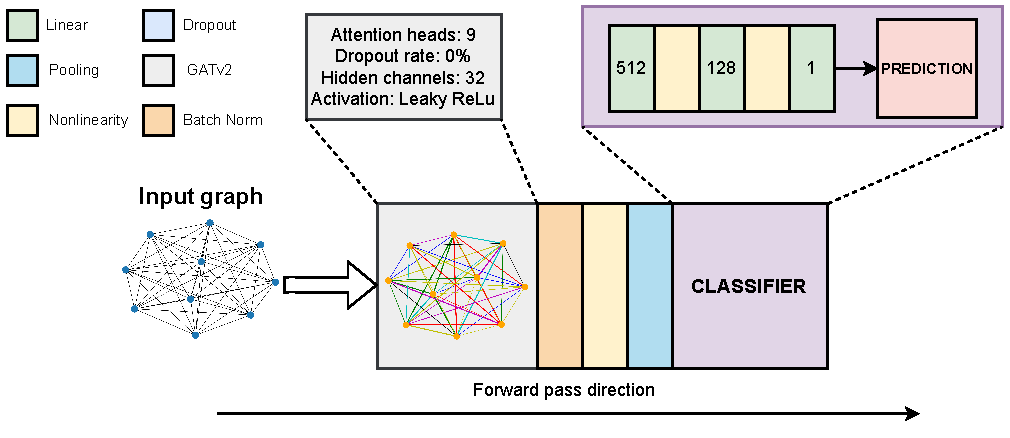
\includegraphics[scale=0.85]{figures/network_final_elsvier.pdf}
    \caption{The graph presenting final network architecture. Numbers in the blocks denote the number of neurons and probability for fully-connected and dropout layers respectively. In this experiment, the nonlinearity used was Leaky ReLu.
    }
    \label{fig:final-network}
\end{figure}



\subsection{Final model evaluation}
To further check the results of NAS, we performed an extended evaluation of the final model. We trained the network from scratch, using 10-fold cross-validation, obeying the same stratification and normalization principles as for the previous NAS experiments. For each test subset, we computed AUROC, F1-score, Sensitivity, Specificity, and Balanced Accuracy. The values of these metrics are shown in Tab. \ref{tab:final-runs-metrics}. Also, the confusion matrix is shown in Fig.\ref{fig:conf-matrix}. The model was able to properly separate the classes, indicated by an average AUROC of 0.9786 across all folds. Specificity is also consistently reaching high values across all folds, with a mean value of 94.91\%. Sensitivity shows slightly lower performance, usually below 90\%, with a mean value of 89.82\%. Looking into the confusion matrix, we can see that the model is the most robust in the detection of seizure patterns, incorrectly classifying only 3.12\% of the samples present in all folds. The number of errors grows for interictal and preictal classes, as the two are often mistaken with each other by the model. 8.22\% of preictal samples are classified as interictal, and 11.84\% of the interictal were mistaken with preictal class.

\begin{figure}[hbt]
  \hspace*{\fill}%
  \begin{minipage}[t]{0.45\textwidth}
    \centering
    \vspace{0pt}
    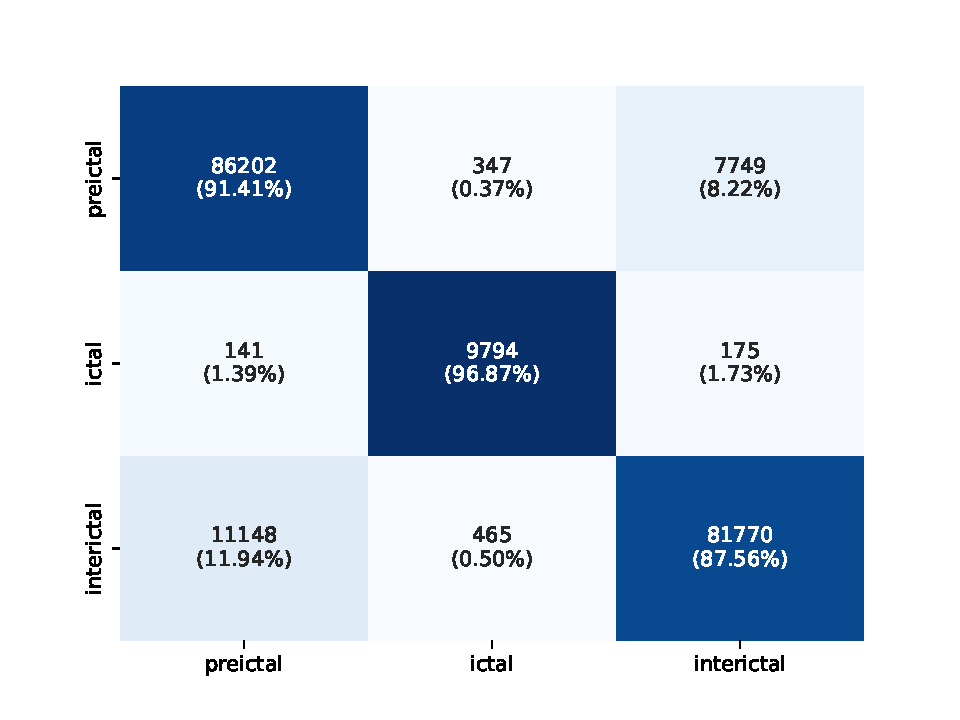
\includegraphics[scale=0.45]{figures/conf_lookback_600.pdf}
    \captionlistentry[figure]{5}
    \label{fig:conf-matrix}
  \end{minipage}%
  \begin{minipage}[t]{0.55\textwidth}
  \centering
  \vspace{0pt}
    \begin{tabular}{|p{0.5in}|p{0.5in}|p{0.5in}|p{0.5in}|p{0.5in}|}
    \hline
    AUROC & F1-score & Sensitivity & Specificity & Balanced \newline accuracy \\
    \hline
    0.9792 & 89.8 & 89.8 & 94.9 & 92.4 \\
    0.9821 & 90.82 & 90.82 & 95.41 & 92.36 \\
    0.983 & 91.25 & 91.25 & 95.62 & 93.24 \\
    0.9786 & 89.92 & 89.92 & 94.96 & 91.67 \\
    0.9741 & 88.56 & 88.56 & 94.28 & 91.36 \\
    0.9862 & 92.33 & 92.33 & 96.17 & 93.71 \\
    0.9738 & 88.49 & 88.49 & 94.24 & 91.12 \\
    0.9714 & 87.79 & 87.79 & 93.9 & 91.04 \\
    0.9829 & 90.99 & 90.99 & 95.49 & 93.11 \\
    0.9743 & 88.25 & 88.25 & 94.13 & 91.08 \\
    \hline
    0.9786 \newline $\pm$ 0.005 & 89.82 \newline $\pm$ 1.52 & 89.82 \newline $\pm$ 1.52 & 94.91 \newline $\pm$ 0.76 & 92.11 \newline $\pm$ 0.99 \\
    \hline
    \end{tabular}

    \captionlistentry[table]{3}
    \label{tab:final-runs-metrics}
    % \label{tab:final-results}
  \end{minipage}
  
  % \addtocounter{table}{-1}
  \addtocounter{figure}{-1}
  % \captionlistentry[table]{A table beside a figure}
    \captionsetup{labelformat=andtable}
    \caption{Results of the final model evaluation. To the right: confusion matrix for predictions made across all folds. Rows refer to ground truth labels, while columns to predicted ones. Percentage values indicate the number of samples classified to a given class relative to the total number of ground truth samples in that class. To the left: metrics describing the performance of the final model on the test sets from consecutive folds. All metrics except AUROC are denoted in percentages. The last row describes the mean for a given metric and its standard deviation.}
    % \label{tab:label}
\end{figure}



% \begin{table}[h!]
% \centering
% \begin{tabular}{|p{0.5in}|p{0.5in}|p{0.5in}|p{0.5in}|p{0.5in}|}
% \hline
% AUROC & F1-score & Sensitivity & Specificity & Balanced \newline accuracy \\
% \hline
% 0.9765 & 91.39 & 91.39 & 95.70 & 93.26 \\
% 0.9703 & 89.17 & 89.17 & 94.59 & 91.37 \\
% 0.9607 & 86.70 & 86.70 & 93.35 & 89.61 \\
% 0.9732 & 91.25 & 91.25 & 95.63 & 92.98 \\
% 0.9745 & 92.00 & 92.00 & 96.00 & 93.62 \\
% 0.9663 & 88.39 & 88.39 & 94.20 & 91.22 \\
% 0.9730 & 90.17 & 90.17 & 95.08 & 92.17 \\
% 0.9702 & 89.60 & 89.60 & 94.80 & 91.63 \\
% 0.9713 & 89.61 & 89.61 & 94.80 & 91.60 \\
% 0.9734 & 90.47 & 90.47 & 95.24 & 92.05 \\
% \hline
% 0.9709 \newline $\pm$ 0.0045 & 89.88 \newline $\pm$ 0.0157 & 89.88 \newline $\pm$ 0.0157 & 94.94 \newline $\pm$ 0.0078 & 91.95 \newline $\pm$ 1.16\ \\
% \hline
% \end{tabular}
% \caption{Performance of the final model on the test sets from consecutive folds. All metrics except AUROC are denoted in percentages. The last row describes the mean for a given metric and its standard deviation.}
% \label{tab:final-run}
% \end{table}
% \FloatBarrier


% \begin{figure}[h]
%     \centering
%     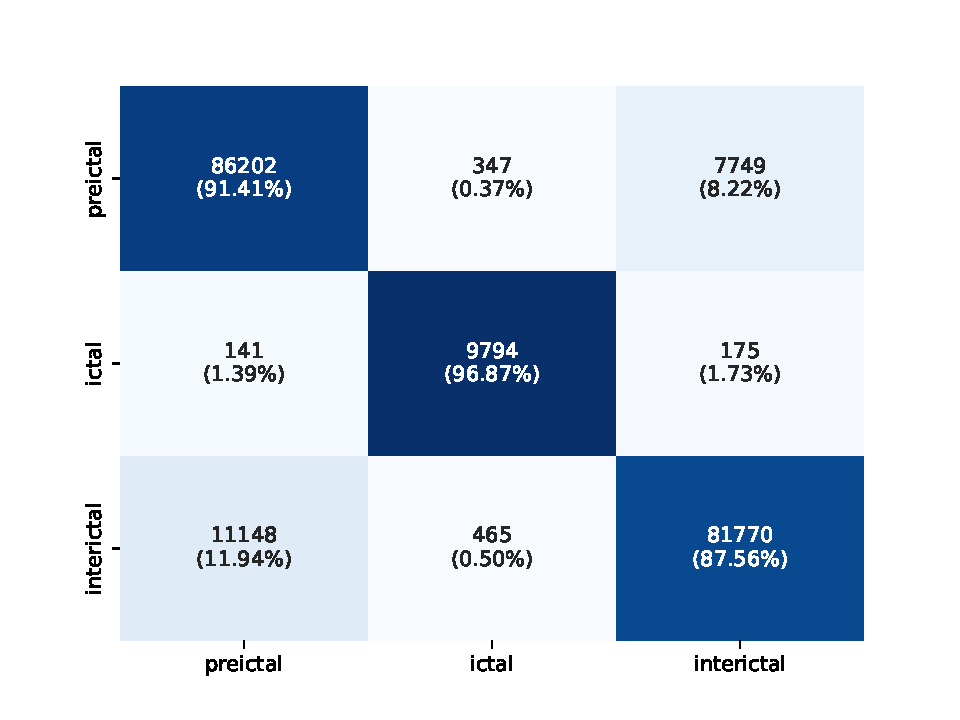
\includegraphics[scale=0.5]{figures/conf_lookback_600.pdf}
%     \caption{Confusion matrix for predictions made across all folds. Rows refer to ground truth labels, while columns to predicted ones. Percentage values indicate the number of samples classified to a given class relative to the total number of ground truth samples in that class.}
%     \label{fig:conf-matrix}
% \end{figure}




\subsection{Predictions explainability}
% The predictions of the final model were also evaluated in terms of explainability using previously described algorithms. The feature importances are visible in Fig. \ref{fig:feature-importance}. The scores indicate that for the interictal period, the Higuchi FD, Hjorth complexity, and $\beta$ band energy are the top three distinctive features, with Hjorth mobility and $\delta$ band energy being nearly equally relevant. In the case of preictal windows, we observe an increase in the relevance of line length, which became the second most relevant feature for the classification. Major changes can be seen when making a classification of the ictal periods. Line length, along with Katz FD is shown to be the most relevant, with other features losing their influence.
The predictions of the final model were also evaluated in terms of explainability using previously described algorithms. The feature importances are visible in Fig. \ref{fig:feature-importance}. Looking at the left subplot, we can see that for the interictal periods, all used features have nearly identical importance. For the preictal period, we can see that there is a major change in the relevance of all features, with Higuch FD, Theta band energy, and Hjorth mobility being the most relevant ones. The importance of features for detecting ictal periods also presents a major change in comparison to interictal periods. Also, a difference exists between preictal and ictal periods, with Katz FD gaining relative importance and Higuch FD losing it in the ictal periods. These changes are also explicitly shown in the right subplot, which describes the absolute difference between ictal and preictal, interictal and ictal, and preictal and ictal periods.

The edge attention scores for every class are shown in Fig. \ref{fig:connectivity}. An increase in the number of relevant edges from the interictal to the preictal to the ictal period is coherent with clinical knowledge, as seizures often spread across the cortex from the source, and overall connectivity increases. Notably, patterns allowing for distinction between the classes emerge. For the preictal samples, the edge between channels F3-T8 disappears, unlike for other periods. In the ictal class, highly relevant for interictal and preictal classes edge Fz-Cz loses its importance. Also, some areas are strongly connected across all classes, namely O2-F3, P7-F7, and O2-P4-P8. We leave extended evaluation of these patterns for future work.

% The changes in functional connectivity based on learned attention coefficients are shown in Fig. \ref{fig:connectivity}. An increase in functional connectivity from the interictal to the preictal to the ictal period indicates a growing synchronization of cortical activity. This is coherent with clinical knowledge, as seizures often spread across the cortex from the source. Also, some regions consistently receive high attention coefficient values, namely O2-F3, P7-F7, and O2-P4-P8. We speculate that areas may be somehow related to epileptic focus, which we leave out for later investigations. Furthermore, these changes
% in connectivity are potentially useful for distinguishing the
% seizure EEG periods, which also require further examination.


\begin{figure}[h!]
	\centering
	\begin{subfigure}{0.45\linewidth}
            \centering
		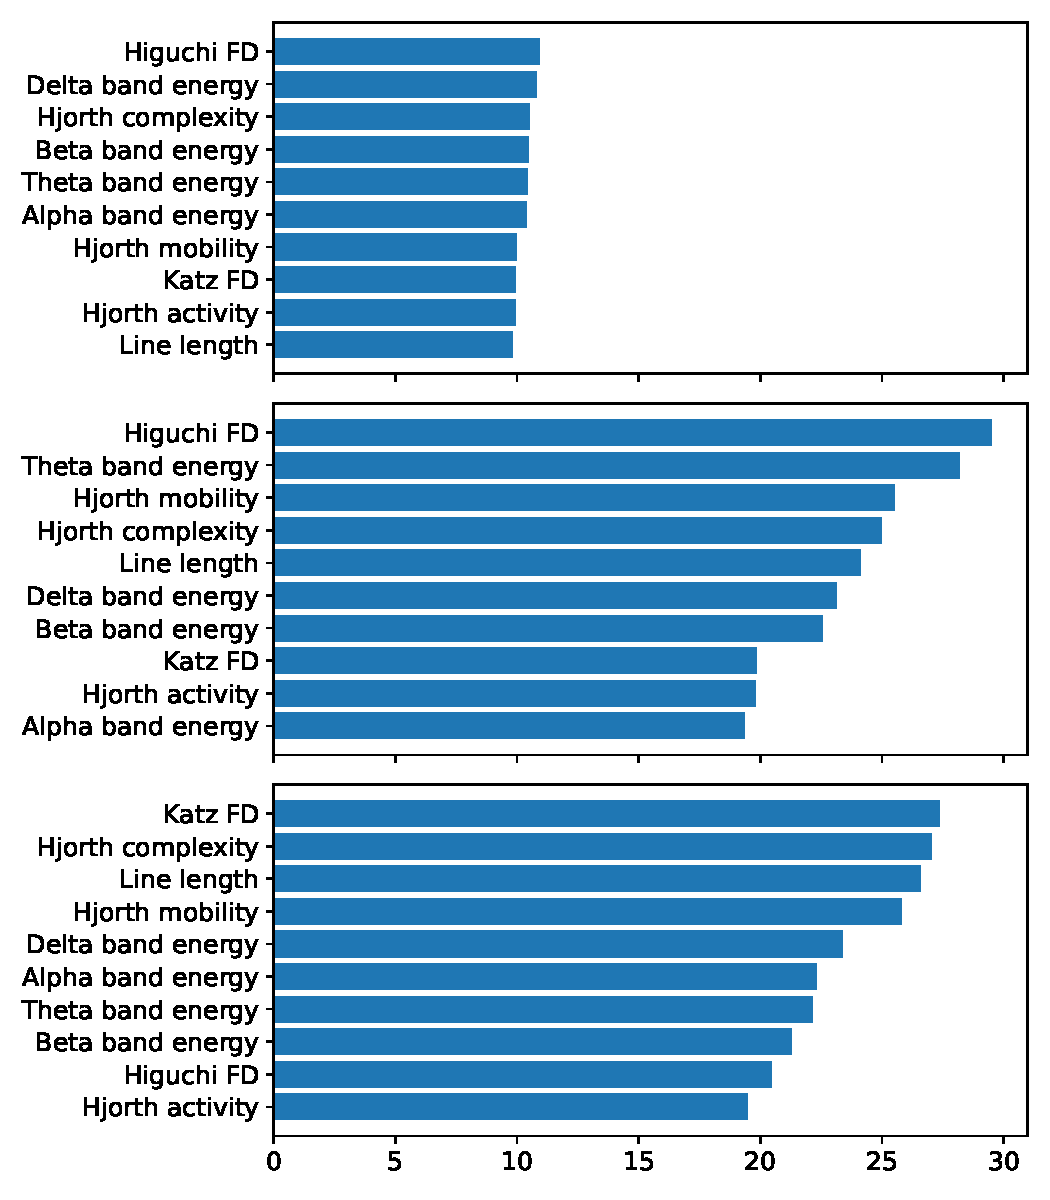
\includegraphics[scale=0.4]{figures/feature_importance_600.pdf}
		
		\label{fig:feature-importance-overall}
	\end{subfigure}
	\begin{subfigure}{0.45\linewidth}
            \centering
		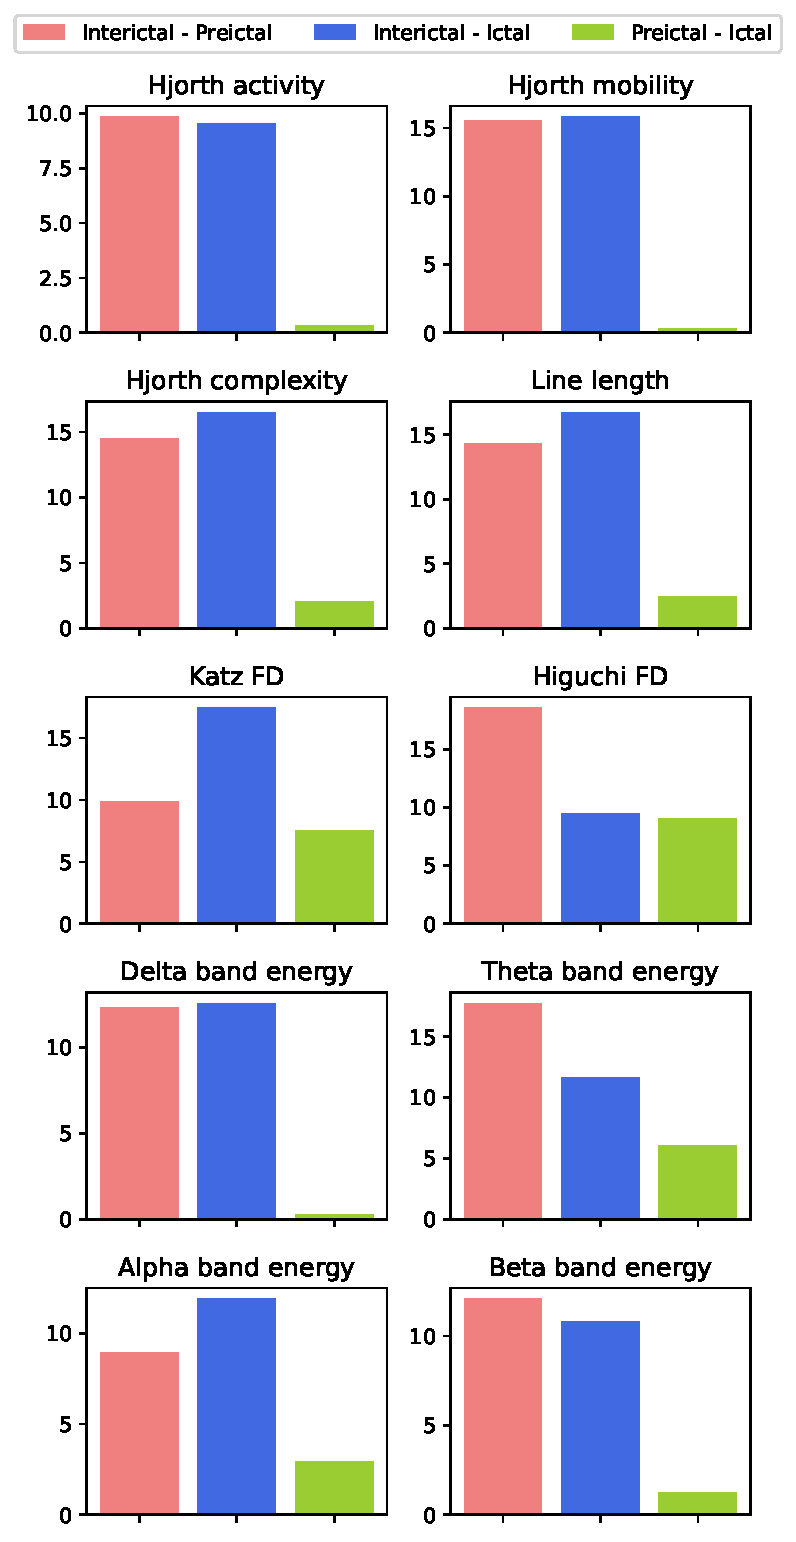
\includegraphics[scale=0.4]{figures/feature_importance_diffs_600.pdf}

		\label{fig:feature-importance-diffs}
	\end{subfigure}
	\caption{Plots showing the analysis of feature importance. To the right: average node feature importance scores obtained from predictions on every sample across all folds. Top: interictal class, middle: preictal class, bottom: ictal class. Left: Differences in importance scores between predictions
for chosen classes. Note that the score values are abstract and unitless. They therefore should be evaluated only relative to the other values obtained within the same set of experiments regarding one model.}
	\label{fig:feature-importance}
\end{figure}
 
\begin{figure}[h]
    \centering
    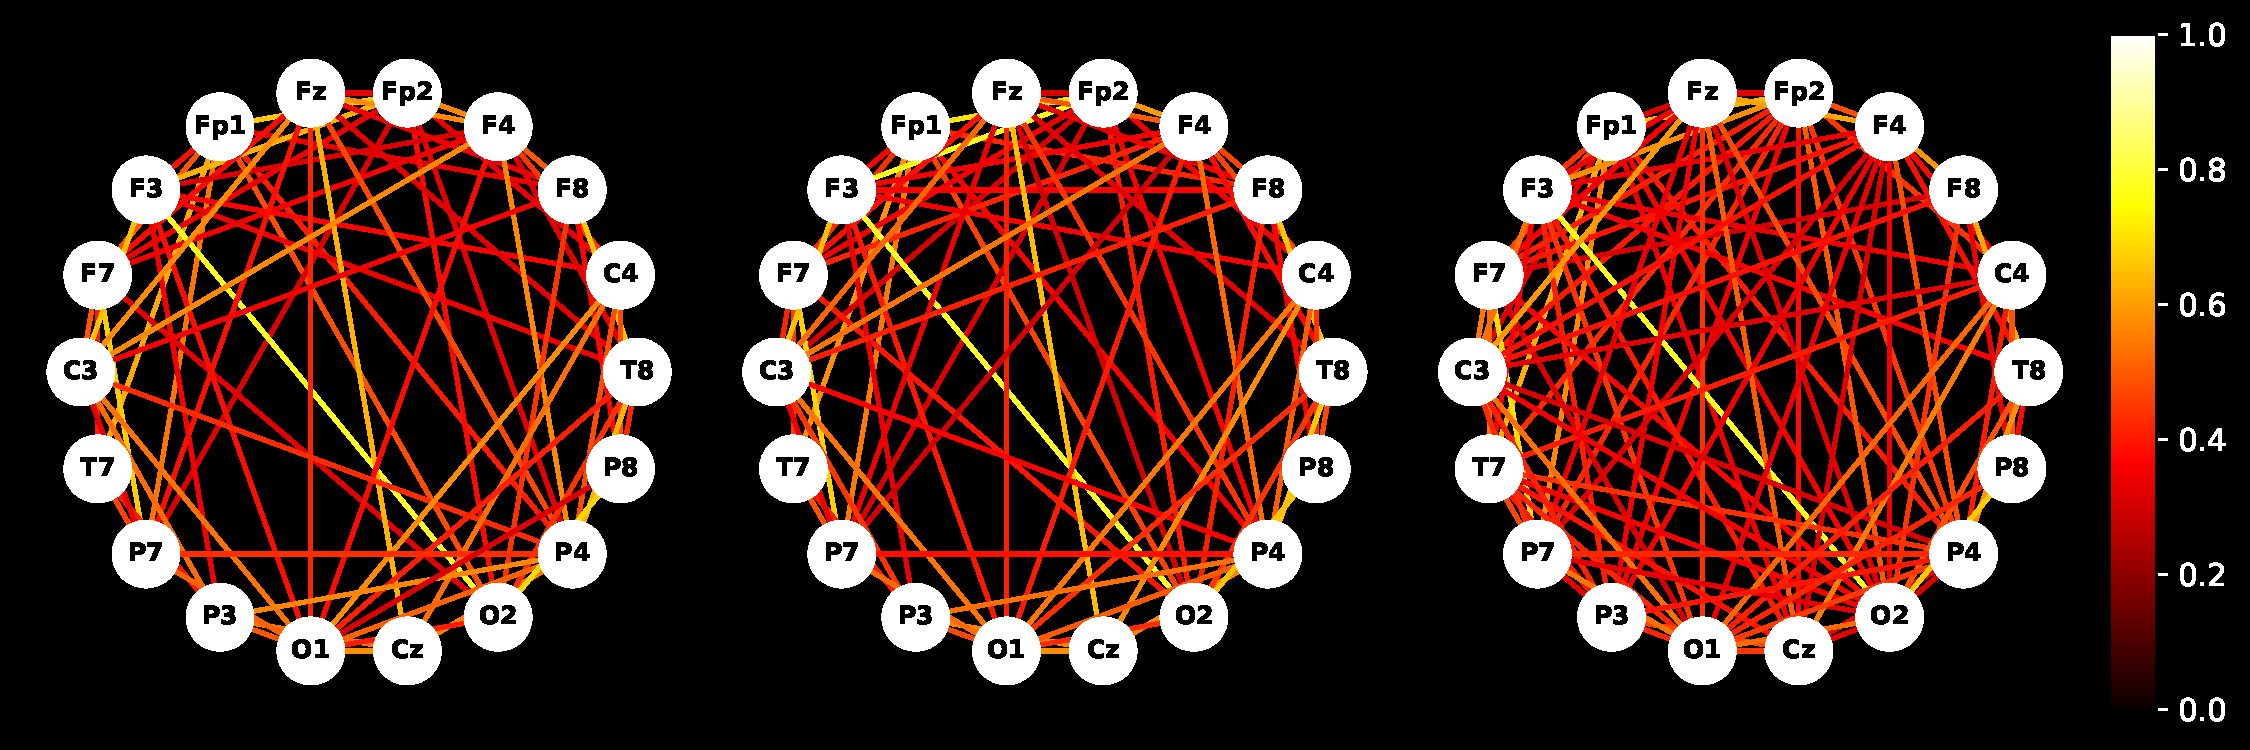
\includegraphics[scale=0.4]{figures/conncectivity_600.pdf}
    \caption{Edge importance scores based on attention coefficients obtained from predictions on every sample across all folds as in Eq. (\ref{edge_explain}). Edges with attention scores below 0.2 are not shown for clarity. Self-loops are not visualized, as we were more interested in the inter-region connections. Left: interictal class; center: preictal class; right: ictal class.}
    \label{fig:connectivity}
\end{figure}
\FloatBarrier

\subsection{Evaluating effective prediction horizon}

The evaluation of the network's predictive performance using different lengths of preictal period is shown in Fig.\ref{fig:predictive-horizon}. 
It can be seen that the network can consistently correctly classify the interictal samples, even with increasing preictal period length. However, we can observe slight performance drops when extending the lookback. For the baseline horizon, the performance is the best, consistently surpassing a 90\% accuracy. Compared to that, horizons of 20 and 30 minutes result in lower performance, with an average value below 90\% and visibly higher variance. The drops start to be more prevalent as the horizon goes beyond the 30 minutes. The closer the times of predictions to the 1-hour to seizure time label, the lower the performance, with some significant drops, even below values of 60\% (see Fig. \ref{fig:predictive-horizon-raw}). However, the architecture's ability to correctly detect seizorous activity remained unaltered regardless of the predictive horizon defined. The features and edges responsible for the model's performance also remained stable through all four settings, with a slight change for the 60-minute scenario (see Appendix \ref{chapter:appendix-2}). %We performed an extended evaluation of the overall performance of these models, as well as computed explainability scores. This evaluation can be found in Appendix \ref{chapter:appendix-2}.

\begin{figure}[h!]
	\centering
	\begin{subfigure}{0.48\linewidth}
		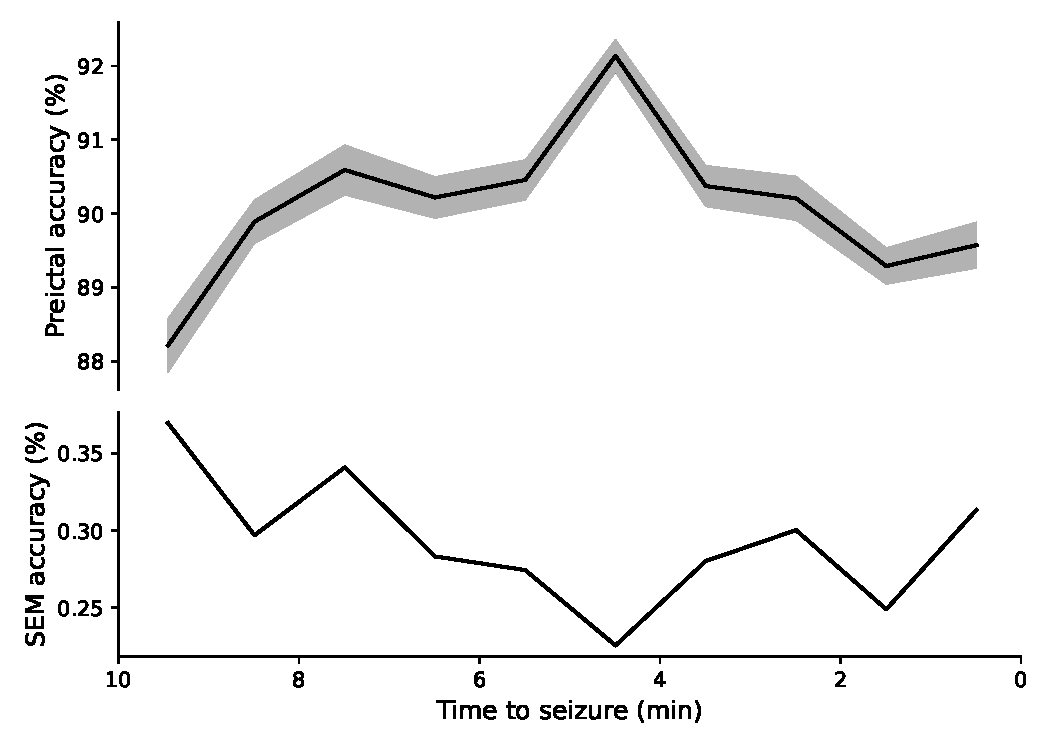
\includegraphics[scale=0.45]{figures/horizon_lookback_600.pdf}
		\caption{10 minutes preictal horizon}
		\label{fig:subfigA}
	\end{subfigure}
	\begin{subfigure}{0.48\linewidth}
		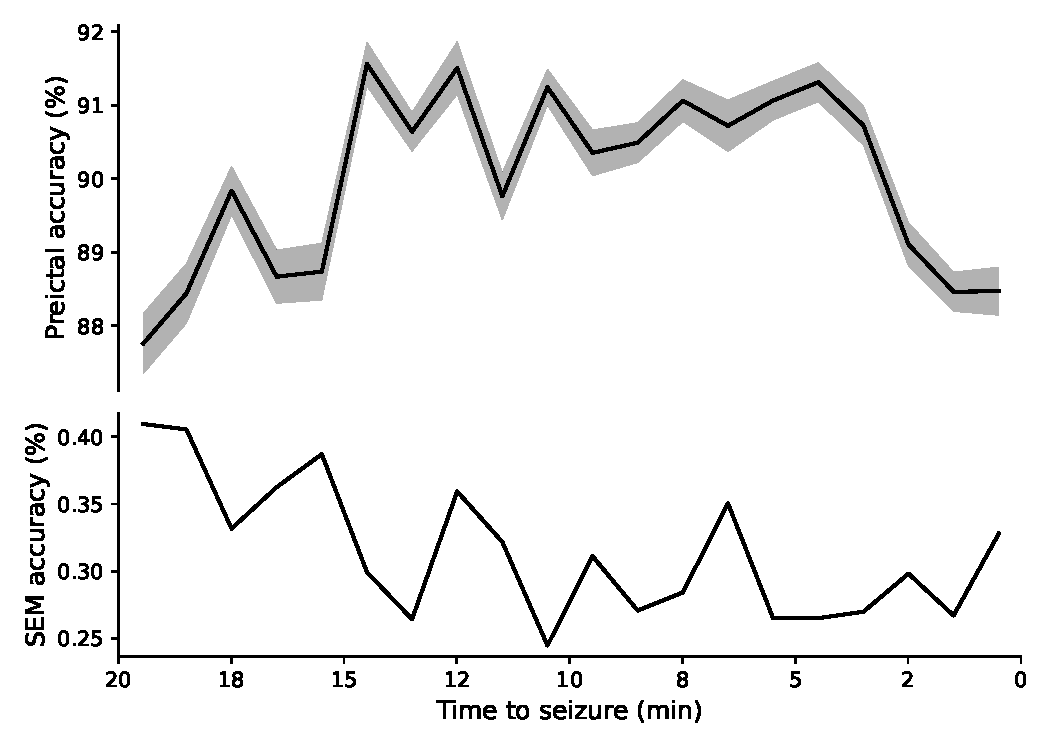
\includegraphics[scale=0.45]{figures/horizon_lookback_1200.pdf}
		\caption{20 minutes preictal horizon}
		\label{fig:subfigB}
	\end{subfigure}
        \vfill
	\begin{subfigure}{0.48\linewidth}
	        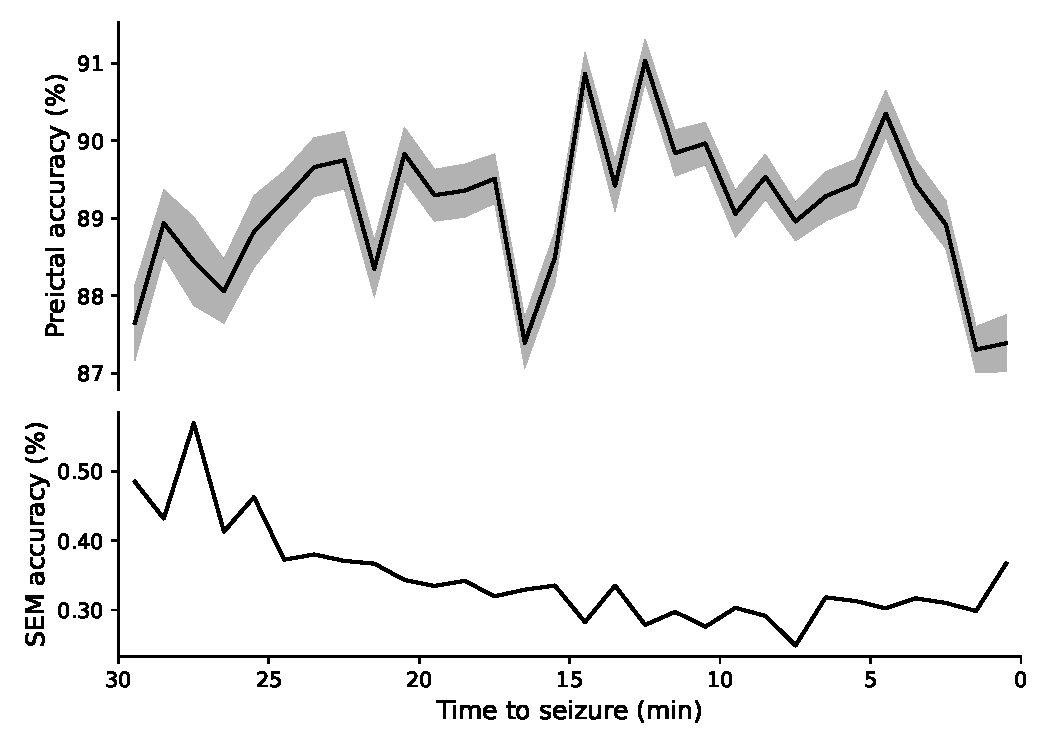
\includegraphics[scale=0.45]{figures/horizon_lookback_1800.pdf}
	        \caption{30 minutes preictal horizon}
	        \label{fig:subfigC}
         \end{subfigure}
         \begin{subfigure}{0.48\linewidth}
	        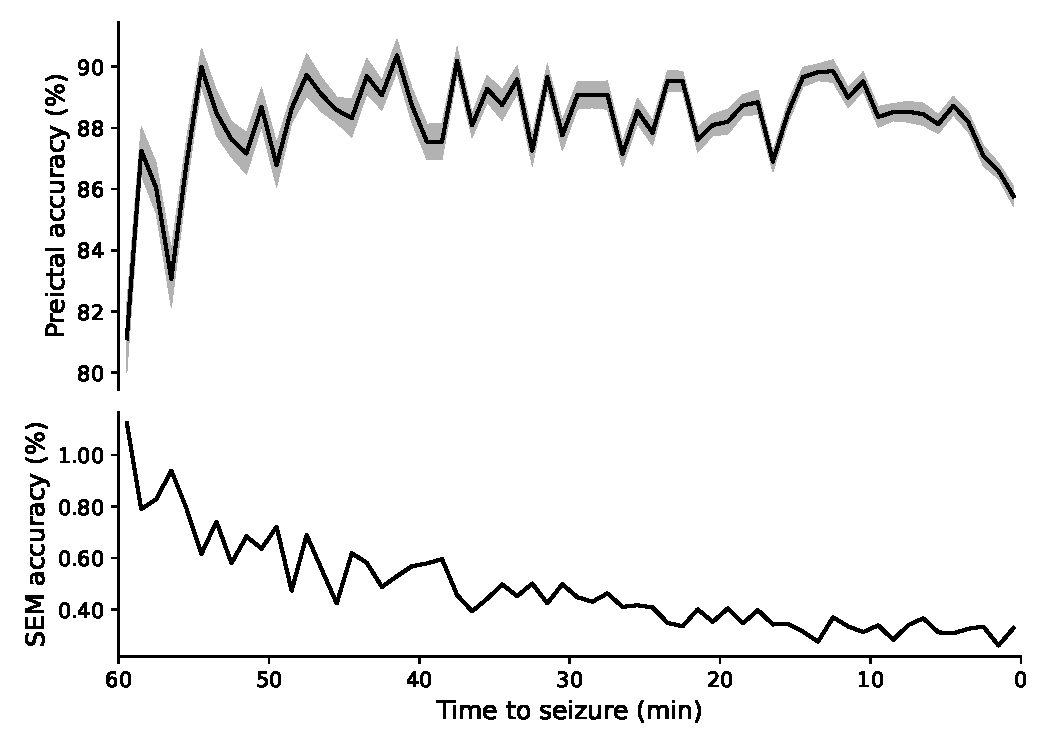
\includegraphics[scale=0.45]{figures/horizon_lookback_3600.pdf}
	        \caption{60 minutes preictal horizon}
	        \label{fig:subfigD}
         \end{subfigure}
	\caption{Plots showing the prediction accuracy for preictal class depending on samples' proximity to seizure paired with the standard error of the mean (SEM) accuracies. The plots were obtained by smoothing the original one with a 60-second window, inside which the accuracies were averaged. In the top plots, the black line denotes averaged accuracy values, while the gray area shows the range of $\pm$ 1 SEM. }
	\label{fig:predictive-horizon}
\end{figure}


\section{Discussion}
In this work, an extensive study on GNN-based epileptic EEG classification was performed. We examined the existing literature, noting that there are vast limitations in terms of data pre-processing as well as experimental methodologies.

First, we explored the problem of data filtering and class balancing. Available automatic methods of artifact removal have not reached satisfying results or we were unable to use them due to noise present in the data. Due to this fact, we proposed our method based on filtering and PCA, then showed its superiority over simple pre-processing methods found in literature, where just high-pass filtering \cite{JiaEfficientGraphConv, he2022gatblstm} or no pre-processing is used \cite{jibon2023gcndnn}. Surprisingly, extensive pre-processing is not a standard approach in the research in this domain, as the performance increases obtained are significant. We hope that our findings will spark additional interest in this area.

Then, we also explored the methods to mitigate the class imbalance. We found that overlapping the extracted windows as well as weights used in the loss function improved the network performance. This provides an important insight for future researchers exploring this problem, as naive usage of some common methods, such as undersampling or oversampling led to performance deterioration. However, observed negative changes were insignificant, which potentially marks those methods as obsolete. On the other hand, proper choice of imbalance handling can help to improve the results even further.

These findings were incorporated into the next experiments where NAS was performed. Here, we expanded our approach to data extraction by using new methods to construct the graphs and extract node features. We show that NAS led to significant gains in the model's performance, with the approach using proposed handcrafted features performing better than when evaluating only power spectrum as node features.

The found configuration of the model was evaluated extensively using 10-fold stratified cross-validation, using metrics that are suitable for dealing with problems of imbalanced data classification. We show that the model can properly separate the classes across all folds, although there is a relatively high incidence of mistaking the interictal class with the preictal one. Although the comparison between methods is difficult due to the aforementioned problems of approach standardization, the obtained performance of average 0.9695 AUROC seems to be competitive with the solutions of similar problems found in the state-of-the-art literature, where authors usually report AUROC above 0.9 \cite{he2022gatblstm, JiaEfficientGraphConv, ZhaoGraphFocalLoss}. The confusion matrix shows that the model can correctly classify most of the ictal samples with 96.54\% of samples classified correctly. The errors occur mostly when discriminating between preictal and ictal classes, with 12.06\% of interictal samples classified incorrectly as preictal and 8.97\% of preictal ones as interictal. These errors may occur due to the labeling criteria used when creating the dataset. Experts marked a period as ictal if the pathological activity lasted 6 seconds or longer. Possibly, some seizurous activity patterns are present in preictal/interictal samples, leading to inconsistencies during the training of the network. Nevertheless, despite these problems, the relatively small number of patients, and their heterogeneity, the model reached satisfying performance.

Transparency in computational medicine must be a requirement for any model to be trusted; thus, explainable AI workflows need to be incorporated. We have proposed two different methods that can be incorporated easily into the realm of AI-based analyses of EEG signals. By modeling the signal as a graph, the non-trivial relationships between electrodes can be unmasked and weighted based on their contribution to the final output of the model. 
We performed the experiments to determine which of the node features used was the most relevant to the prediction. We also use obtained attention scores from GATv2 layers to establish the edge importance, therefore providing some guidance about the changes in brain connectivity for different EEG periods. We observed that used features have predictive properties for preictal and ictal periods, with Higuchi FD and line length being the most descriptive for them respectively. When classifying interictal periods none of the features turned out to be more informative than the others, possibly indicating that to improve performance in this class additional features should be incorporated.
Changes in edge importance between classes seem to confirm the medical domain knowledge, with increased connectivity between all regions of the brain when seizure is nearing. The observed changes open a possibility to be useful as features for performing classification themselves. From the clinical standpoint, we speculate that these scores can have potential in seizure focus localization, as some strongly interconnected regions appear across all sample types, possibly indicating the brain regions where pathological activity is visible the most.

Importantly, an accurate and reliable seizure recognition automated pipeline does not necessarily imply a trustworthy prediction of the time remaining until the next epileptic episode, not trivially at least. A naïve approach to the prediction of future seizures would imply the minimization of a cost function incorporating the time to seizure label – for example, by minimizing the mean squared error between the true and predicted time. However, such a prediction based only on a given short time window poses a significant challenge, even for seasoned clinicians. Instead, we propose to take an indirect approach by evaluating the capacity of our model to maintain the accuracy at detecting preictal activity. Even after increasing the predictive horizon to 60 minutes before seizure onset, the accuracies remained above the 85\% threshold in all temporal scales, dropping slightly toward the 40-50 minutes horizon.  

% Lastly, we evaluate the model's ability to predict the incoming seizure via correctly detecting the preictal samples. We checked this performance for different lengths of the preictal period - 10, 20, 30, and 60 minutes. The model was able to maintain its high accuracy for preictal sample prediction, although it is visible that when the predictive horizon is increased, the performance starts to deteriorate. Another promising observation is that the model maintains the predictive performance in the proximity of the seizure (below 20 minutes before the event) despite increasing the lookback time. 
Preictal activity, as the name suggests, is followed by pathological periods of brain activity. Conceptually, if the model can accurately predict preictal activity up to 1 hour before the seizure occurs, it follows that the first preictal prediction is indicative of the time to seizure. Of course, this simplification needs to be further evaluated and refined. For example, in the testing phase, samples could be sequentially forwarded into the classifier, and a posterior belief of the time to seizure given the predicted preictal class could be computed. Formally,
\begin{equation*}
    P(time|preictal) \propto (preictal|time)P(time), 
\end{equation*}
where $time$ is a given time window, $P(time)$ is a prior belief, and $P(preictal|time)$
is the likelihood of predicting preictal activity given an unknown time. The former might take several forms, while the latter could be extracted from the trained model by evaluating the ability of the AI system to maintain accuracies across different horizons (Fig. \ref{fig:predictive-horizon}). Moreover, the posterior belief could be constantly updated to decrease the uncertainty of the model (e.g., via a Gaussian process or partially observable Markov decision processes \cite{kaelbling1998planning}). Needless to say, this approach requires further investigation.

Other parts of this work can also be expanded, addressing some of the limitations.
The dataset contained a small number of subjects compared to those present in cohort studies, it is thus necessary to do so to finally confirm the clinical applicability. Secondly, a more precise evaluation of the different filtering frequencies and PCA usage can be performed - the frequency threshold and the number of PCA components can be tuned. There are some findings in the literature that high-frequency oscillations can have diagnostic value in detecting ictal and preictal patterns \cite{jung2019hfoepilepsy} and they should be maintained in the signal.
NAS search space can also be expanded - the architecture would probably also benefit from the utilization of some sort of skip connections and varying the number of neurons in the hidden layers to increase its capacity.



\section{Conclusions}

In this work, we present a comprehensive, end-to-end approach for creating graph deep learning models for EEG classification and seizure prediction in epileptic patients. Starting from the signal filtering, we show that denoising can significantly improve the network's performance. We propose a denoising method for artifact removal based on PCA, showing its effectiveness in increasing the classifier's performance. We also provide insight into class imbalance handling methods, showing that their careful usage can increase the model's performance even further. Next, we use Bayesian architecture search to optimize the model's architecture and training hyperparameters, allowing the model to reach robust performance across 10 testing folds. Then, we use explainability algorithms to compute the feature and edge importances, showing changes that shed light on the decision boundaries learned by the model. Lastly, we evaluate the model's capability to predict the seizure via the classification of pre-ictal samples. We show that the model maintains high performance when classifying preictal samples coming from the period up to 60 minutes before the seizure. We hope that these findings will help to deploy such systems in real clinical scenarios.

\appendix

\section{Appendix 1}
\label{chapter:appendix-1}
\subsection{Fast Fourier Transform}
For the experiments to determine optimal pre-processing, the time series were transformed into a vector representing power spectral density:
\begin{equation}
    S_k= |X_k|^{2},
\end{equation}
where $S(f_k)$ is a power spectral density at frequency $f_k$ and $X(f_k)$ is a value of
Fourier coefficient at frequency $f_k$. Fourier coefficients are obtained by applying the Discrete Fourier Transform (DFT) to the input signal x(t). The k-th coefficient is obtained by:
\begin{equation}
    X_k = \sum_{i=0}^{N-1}x_i e^{-ki\frac{2\pi j}{N}}, k \in {0,1,2, ..., N-1},
\end{equation}
where $N$ is the length of the sample, $N$ is the sample length, $e$ is an Eurler's number and $j$ is the imaginary number.
The DFT was computed using Fast-Fourier Transform (FFT) algorithm introduced by \cite{Cooley1965FFT} and
implemented in the Python library Numpy 1.25.2 \cite{harris2020numpy}. Noteworthy, in the case of this paper the coefficients obtained with DFT were normalized with $N$.
\subsection{Phase Locking Value}
The Phase Locking Value (PLV) \cite{bruna2018plv} is a measure used when constructing adjacency matrices for the samples in architecture search experiments. PLV between two signals $i$ and $j$ is defined as:
\begin{equation}
    PLV_{i,j} = \frac{1}{N}|\sum_{n=1}^{N}{e^{-j(\phi_i(n)-\phi_j(n))}}|,
\end{equation}
where $\phi(n)$ is the instantaneous phase of each signal at timestep $n$.
\subsection{Hjorth Parameters}
Hjorth parameters \cite{hjorth1970params} are indicators of statistical properties of the analyzed timeseries. Activity, which is denoted simply as a variance of the observed timeseries:
\begin{equation}
    A(x(t)) = \text{var}(x(t)).
\end{equation}
It allows us to measure if the high-frequency components occur often in the signal.
Mobility, expressed as:
\begin{equation}
    \text{Mob}(x(t)) = \sqrt{\frac{A(x'(t))}{A(x(t))}},
\end{equation}
shows the mean frequency. Lastly, Complexity is expressed as:
\begin{equation}
    \text{Compl}(x(t))=\frac{\text{Mob}(x'(t))}{\text{Mob}(x(t))},
\end{equation}.
This measure shows the similarity of the measured signal to the pure sine wave.
\subsection{Line length}
Line length is calculated as a normalized running sum of the absolute differences between consecutive signal samples within a chosen time window, providing a measure of signal variability. It is expressed as:
\begin{equation}
    L(x(t))= \sum_{i=1}^{N-1}(|x_{i+1} - x_{i}|),
\end{equation}
where $N$ is the number of samples in a time window. In our experiments, we use a normalized version, which is simply dividing the obtained line length by a number of samples in the window $L_n(x(t)) = \frac{1}{N-1}L(x(t))$.

\subsection{Fractal dimensions}
Intuitively, fractal dimension (FD) of a time series can be understood as a measure of the deviation of a signal from a 1D straight line towards 2D plane covering the entire analyzed time window domain.
Katz FD of a signal can be denoted as:
\begin{equation}
    D_{Katz}(x(t)) = \frac{\log_{10}(N)}{\log_{10}(\frac{d}{L(x(t))})+\log_{10}(N)},
\end{equation}
where $d$ is a \textit{diameter} defined as the distance from the first point in the analyzed time window and the one that leads to maximization of the distance:
\begin{equation}
    d = \text{max }_{t \in N, t\neq{t_1}}|x(t_1) - x(t)|
\end{equation}

On the other hand, the Higuchi formula defines the approach to FD estimation in the following way:
Considering time series $X$ with the $N$ discrete data points, we construct $k$ new time series $X^{k}_{m}$:

\begin{equation}
    X^{k}_{m}=\{ X(m),X(m+k),X(m+2k),..., X(m+Z), 
\end{equation}
where $m \in \{1,2,...,k\}$ denotes the initial starting data point, $k$ describes the time interval between points and $Z=\lfloor \frac{N-m}{k} \rfloor)\}$. In our study, we set $k=10$. Next, the average line length is computed for each new curve $ X^{k}_{m}$, given by:
\begin{equation}
    L_m(k) = \frac{\sum_{i=1}^{Z} |X((m+ik)-x(m+(i-1)k|(n-1)}{Z k}
\end{equation}
Finally, the sum of the average length is computed:
\begin{equation}
    L(k)=\frac{1}{k}\sum_{m=1}^{k} L_{m}(k).
\end{equation}
Obtaining the curve of $\text{ln}(L(k))$ against $\text{ln}(k^{-1})$, the slope of the best-fitting linear function obtained by the least squares method is the searched approximation of FD. 
\subsection{Signal energy}

The energy of a discrete-time signal of length N is defined as:
\begin{equation}
    E(x(t)) = \sum_{n=0}^{N}x(t_n)^{2} 
\end{equation}
In this work, we calculated the energy of a given time series associated with an EEG channel for different energy bands by first applying the 4th-order Butterworth filter to include only the analyzed frequency band. The frequency bands were defined as follows: delta (0.5 to 4 Hz), theta (4 to 8 Hz), alpha (8 to 13 Hz) and beta (13 to 29 Hz). The lower limit of the delta band and the upper one of the beta band were chosen to fall within the filtering band ranges (0.5 to 30 Hz) obtained in the pre-processing step.

\section{Appendix 2}
\label{chapter:appendix-2}
\subsection{Metrics and performance evaluation}
We performed additional evaluations of the models trained for different preictal lookback horizons. The results are shown in Tab.\ref{tab:metrics-lookback-1200} to \ref{tab:metrics-lookback-3600} and Fig.\ref{fig:conf-matrix-1200} to \ref{fig:conf-matrix-3600}. Metrics values show that the model can maintain its performance with increasing preictal lookback. These results are promising, as they indicate that the model found by the NAS was not overturned to perform only on a certain data subset. It also shows the potential usefulness of the model in seizure prediction tasks with long predictive horizons.
Similar things can be seen examining the confusion matrices, as the performance for given classes did not change significantly between the horizons. It is visible that the model maintained a seizure detection perspective, where the number of samples stays roughly the same, whereas, for the remaining classes, it grows significantly. 
\begin{figure}[hbt]
  \hspace*{\fill}%
  \begin{minipage}[t]{0.45\textwidth}
    \centering
    \vspace{0pt}
    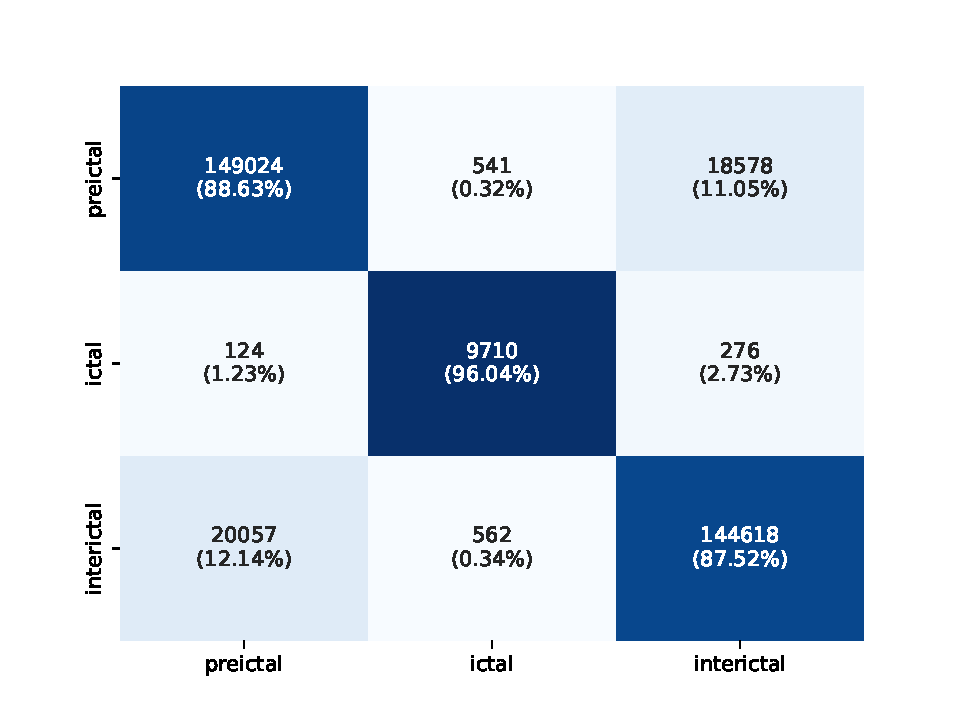
\includegraphics[scale=0.45]{figures/conf_lookback_1200.pdf}
    \captionlistentry[figure]{5}
    \label{fig:conf-matrix-1200}
  \end{minipage}%
  \begin{minipage}[t]{0.55\textwidth}
  \centering
  \vspace{0pt}
    \begin{tabular}{|p{0.5in}|p{0.5in}|p{0.5in}|p{0.5in}|p{0.5in}|}
    \hline
    AUROC & F1-score & Sensitivity & Specificity & Balanced \newline accuracy \\
    \hline
    0.9763 & 89.14 & 89.14 & 94.57 & 92.03 \\
    0.9731 & 88.33 & 88.33 & 94.17 & 91.32 \\
    0.9769 & 89.59 & 89.59 & 94.79 & 92.04 \\
    0.9766 & 89.32 & 89.32 & 94.66 & 91.78 \\
    0.9775 & 89.44 & 89.44 & 94.72 & 92.0 \\
    0.9841 & 91.57 & 91.57 & 95.78 & 93.68 \\
    0.9814 & 90.43 & 90.43 & 95.21 & 92.46 \\
    0.9669 & 86.77 & 86.77 & 93.39 & 90.11 \\
    0.9826 & 90.96 & 90.96 & 95.48 & 93.05 \\
    0.9759 & 89.04 & 89.04 & 94.52 & 92.02 \\
    \hline
    0.9771 \newline $\pm$ 0.0049 & 89.46 \newline $\pm$ 1.35 & 89.46 \newline $\pm$ 1.35 & 94.73 \newline $\pm$ 0.68 & 92.05 \newline $\pm$ 0.96 \\
    \hline
\end{tabular}

    \captionlistentry[table]{3}
    \label{tab:metrics-lookback-1200}
    % \label{tab:final-results}
  \end{minipage}
  
  % \addtocounter{table}{-1}
  \addtocounter{figure}{-1}
  % \captionlistentry[table]{A table beside a figure}
    \captionsetup{labelformat=andtable}
    \caption{Results of the final model evaluation for preictal horizon of 20 minutes. To the right: confusion matrix for predictions made across all folds. Rows refer to ground truth labels, while columns to predicted ones. Percentage values indicate the number of samples classified to a given class relative to the total number of ground truth samples in that class. To the left: metrics describing the performance of the final model on the test sets from consecutive folds. All metrics except AUROC are denoted in percentages. The last row describes the mean for a given metric and its standard deviation.}
    % \label{tab:label}
\end{figure}
\FloatBarrier
\begin{figure}[hbt]
  \hspace*{\fill}%
  \begin{minipage}[t]{0.45\textwidth}
    \centering
    \vspace{0pt}
    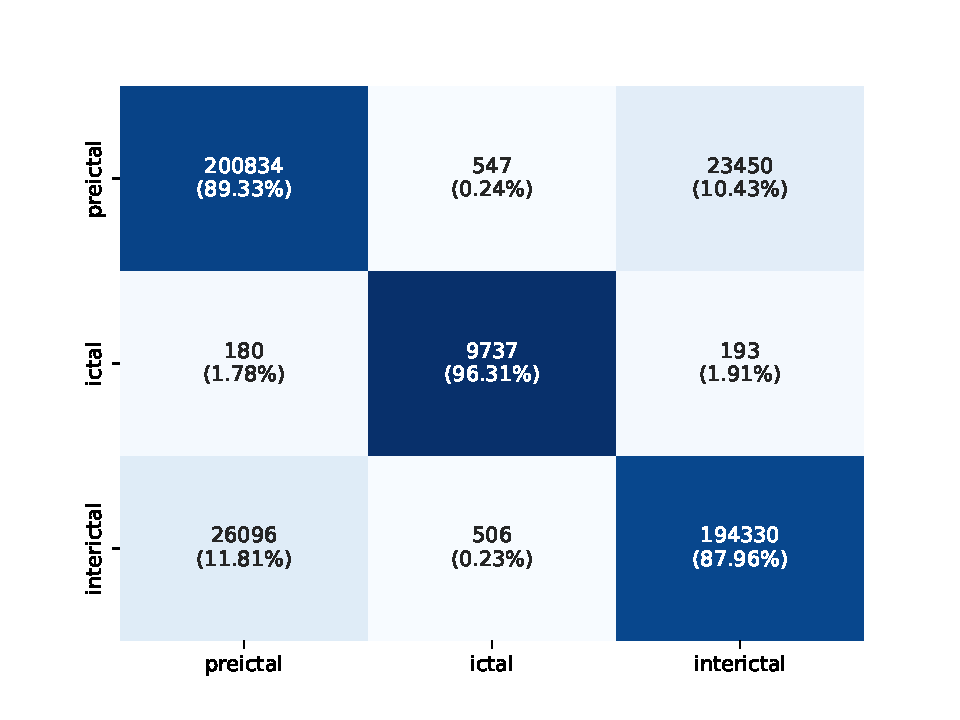
\includegraphics[scale=0.45]{figures/conf_lookback_1800.pdf}
    \captionlistentry[figure]{5}
    \label{fig:conf-matrix-1800}
  \end{minipage}%
  \begin{minipage}[t]{0.55\textwidth}
  \centering
  \vspace{0pt}
    \begin{tabular}{|p{0.5in}|p{0.5in}|p{0.5in}|p{0.5in}|p{0.5in}|}
    \hline
    AUROC & F1-score & Sensitivity & Specificity & Balanced \newline accuracy \\
    \hline
    0.9768 & 89.3 & 89.3 & 94.65 & 91.94 \\
    0.9774 & 89.51 & 89.51 & 94.76 & 92.11 \\
    0.9774 & 89.44 & 89.44 & 94.72 & 91.96 \\
    0.9819 & 90.59 & 90.59 & 95.29 & 92.91 \\
    0.9695 & 87.52 & 87.52 & 93.76 & 90.65 \\
    0.9819 & 90.92 & 90.92 & 95.46 & 92.75 \\
    0.9743 & 88.83 & 88.83 & 94.42 & 91.73 \\
    0.9719 & 87.95 & 87.95 & 93.98 & 91.31 \\
    0.976 & 89.18 & 89.18 & 94.59 & 91.91 \\
    0.9729 & 88.29 & 88.29 & 94.15 & 91.35 \\
    \hline
    0.976 \newline $\pm$ 0.004 & 89.15 \newline $\pm$ 1.07 & 89.15 \newline $\pm$ 1.07 & 94.58 \newline $\pm$ 0.54 & 91.86 \newline $\pm$ 0.67 \\
    \hline
\end{tabular}

    \captionlistentry[table]{3}
    \label{tab:metrics-lookback-1800}
    % \label{tab:final-results}
  \end{minipage}
  
  % \addtocounter{table}{-1}
  \addtocounter{figure}{-1}
  % \captionlistentry[table]{A table beside a figure}
    \captionsetup{labelformat=andtable}
    \caption{Results of the final model evaluation for preictal horizon of 30 minutes. To the right: confusion matrix for predictions made across all folds. Rows refer to ground truth labels, while columns to predicted ones. Percentage values indicate the number of samples classified to a given class relative to the total number of ground truth samples in that class. To the left: metrics describing the performance of the final model on the test sets from consecutive folds. All metrics except AUROC are denoted in percentages. The last row describes the mean for a given metric and its standard deviation.}
    % \label{tab:label}
\end{figure}

\begin{figure}[hbt]
  \hspace*{\fill}%
  \begin{minipage}[t]{0.45\textwidth}
    \centering
    \vspace{0pt}
    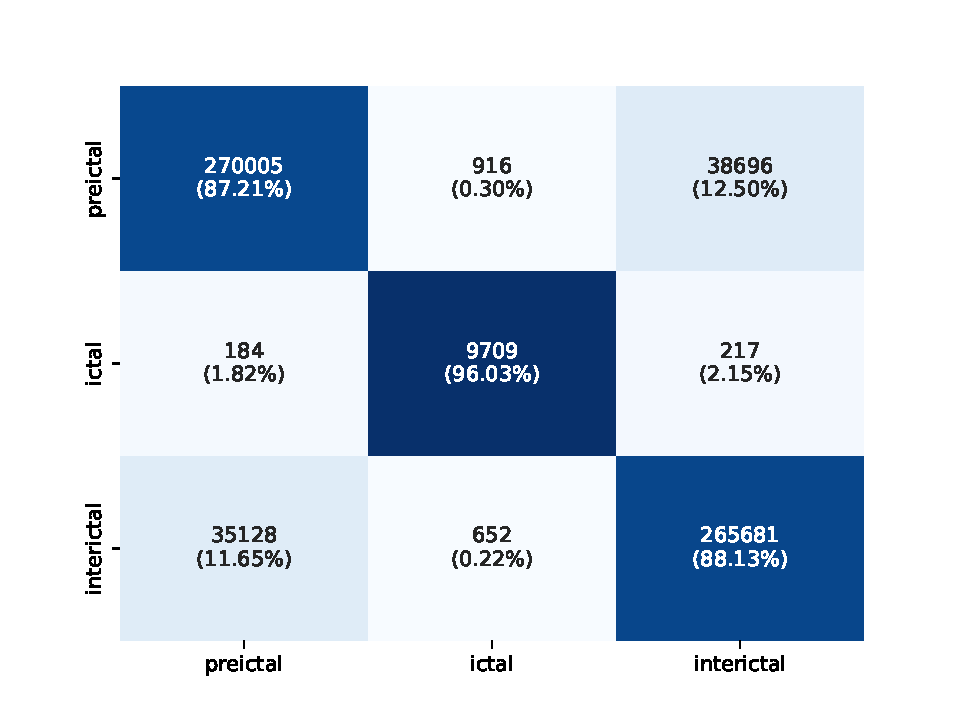
\includegraphics[scale=0.45]{figures/conf_lookback_3600.pdf}
    \captionlistentry[figure]{5}
    \label{fig:conf-matrix-3600}
  \end{minipage}%
  \begin{minipage}[t]{0.55\textwidth}
  \centering
  \vspace{0pt}
    \begin{tabular}{|p{0.5in}|p{0.5in}|p{0.5in}|p{0.5in}|p{0.5in}|}
    \hline
    AUROC & F1-score & Sensitivity & Specificity & Balanced \newline accuracy \\
    \hline
    0.975 & 89.09 & 89.09 & 94.54 & 92.03 \\
    0.9738 & 88.72 & 88.72 & 94.36 & 91.27 \\
    0.9592 & 84.92 & 84.92 & 92.46 & 89.15 \\
    0.9801 & 90.35 & 90.35 & 95.17 & 92.64 \\
    0.9727 & 87.93 & 87.93 & 93.96 & 91.13 \\
    0.9746 & 88.78 & 88.78 & 94.39 & 91.58 \\
    0.9737 & 88.67 & 88.67 & 94.33 & 91.54 \\
    0.9658 & 86.92 & 86.92 & 93.46 & 90.36 \\
    0.9828 & 91.11 & 91.11 & 95.55 & 93.38 \\
    0.9634 & 86.18 & 86.18 & 93.09 & 89.74 \\
    \hline
    0.9721 \newline $\pm$ 0.0073 & 88.27 \newline $\pm$ 1.86 & 88.27 \newline $\pm$ 1.86 & 94.13 \newline $\pm$ 0.93 & 91.28 \newline $\pm$ 1.28 \\
    \hline
\end{tabular}

    \captionlistentry[table]{3}
    \label{tab:metrics-lookback-3600}
    % \label{tab:final-results}
  \end{minipage}
  
  % \addtocounter{table}{-1}
  \addtocounter{figure}{-1}
  % \captionlistentry[table]{A table beside a figure}
    \captionsetup{labelformat=andtable}
    \caption{Results of the final model evaluation for preictal horizon of 60 minutes. To the right: confusion matrix for predictions made across all folds. Rows refer to ground truth labels, while columns to predicted ones. Percentage values indicate the number of samples classified to a given class relative to the total number of ground truth samples in that class. To the left: metrics describing the performance of the final model on the test sets from consecutive folds. All metrics except AUROC are denoted in percentages. The last row describes the mean for a given metric and its standard deviation.}
    % \label{tab:label}
\end{figure}

\subsection{Predictive horizon}
In Fig. \ref{fig:predictive-horizon-raw} we show the raw, unsmoothed accuracies for predicting preictal samples with certain proximity to the seizure event. The trends are still visible, showing that the averaging method does not alter the presented outcomes.
\begin{figure}[h]
	\centering
	\begin{subfigure}{0.48\linewidth}
		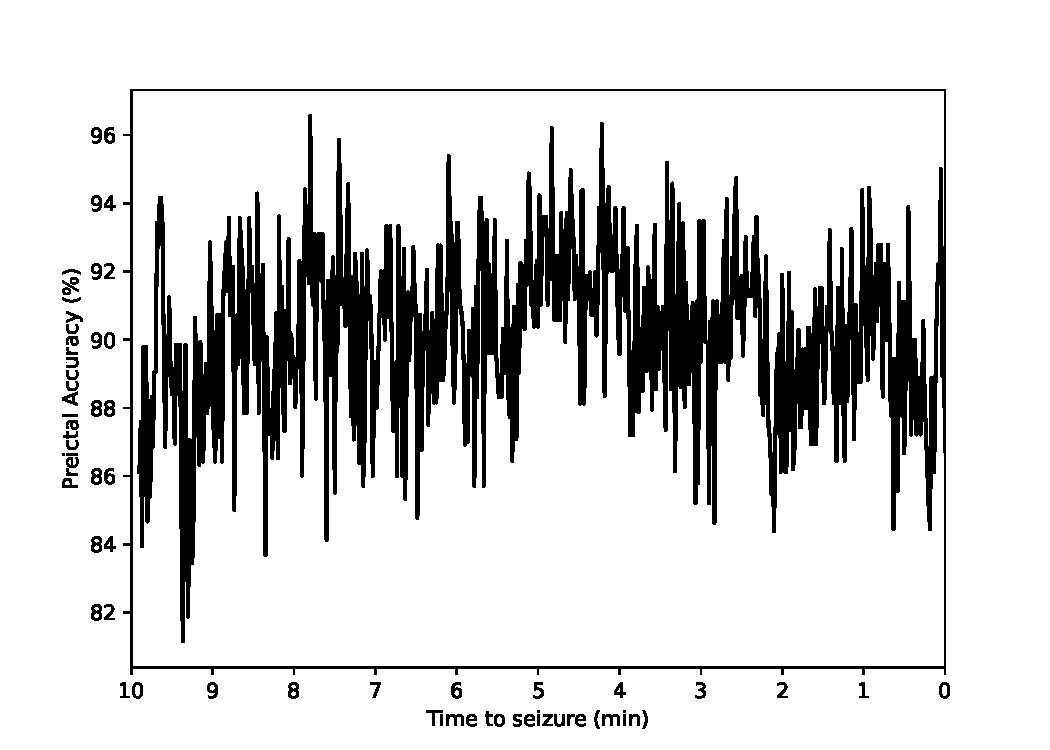
\includegraphics[scale=0.45]{figures/horizon_lookback_600_raw.pdf}
		\caption{10 minutes preictal horizon}
		\label{fig:preictal-accuracy-raw-10min}
	\end{subfigure}
	\begin{subfigure}{0.48\linewidth}
		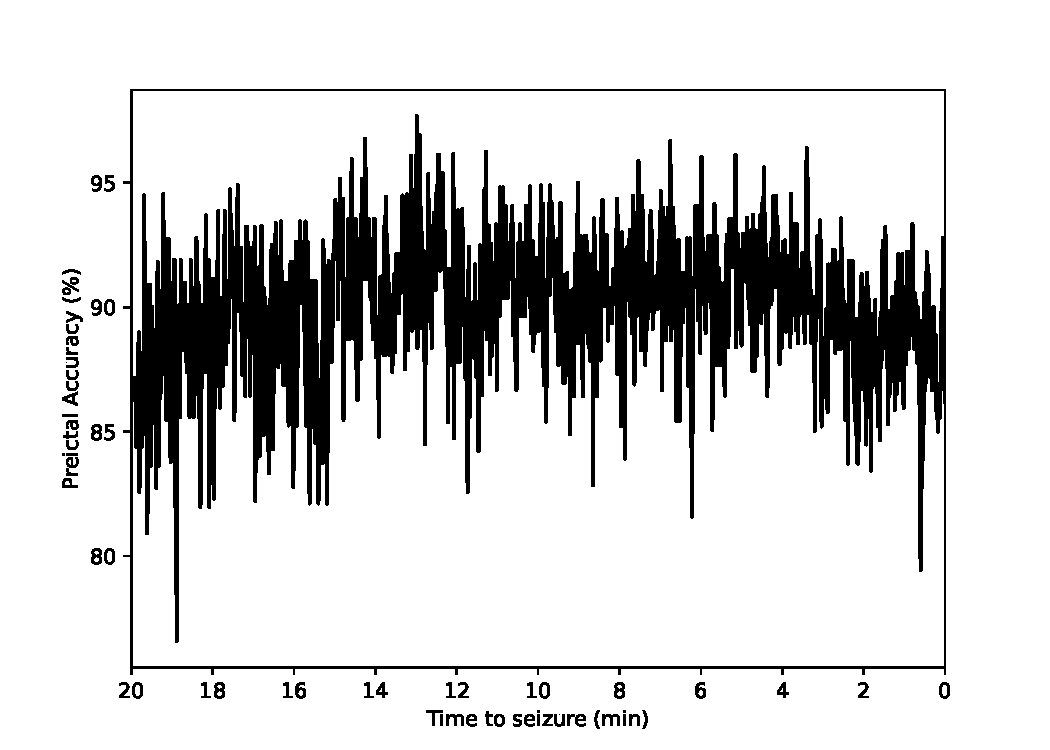
\includegraphics[scale=0.45]{figures/horizon_lookback_1200_raw.pdf}
		\caption{20 minutes preictal horizon}
		\label{fig:preictal-accuracy-raw-20min}
	\end{subfigure}
        \vfill
	\begin{subfigure}{0.48\linewidth}
	        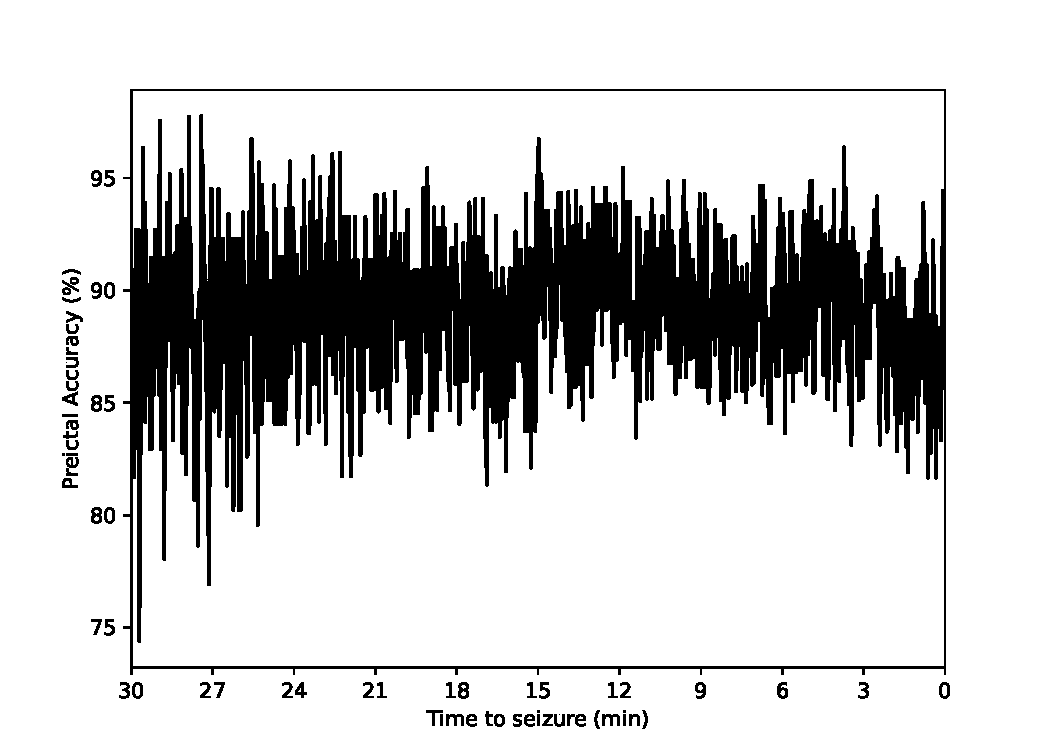
\includegraphics[scale=0.45]{figures/horizon_lookback_1800_raw.pdf}
	        \caption{30 minutes preictal horizon}
	        \label{fig:preictal-accuracy-raw-30min}
         \end{subfigure}
         \begin{subfigure}{0.48\linewidth}
	        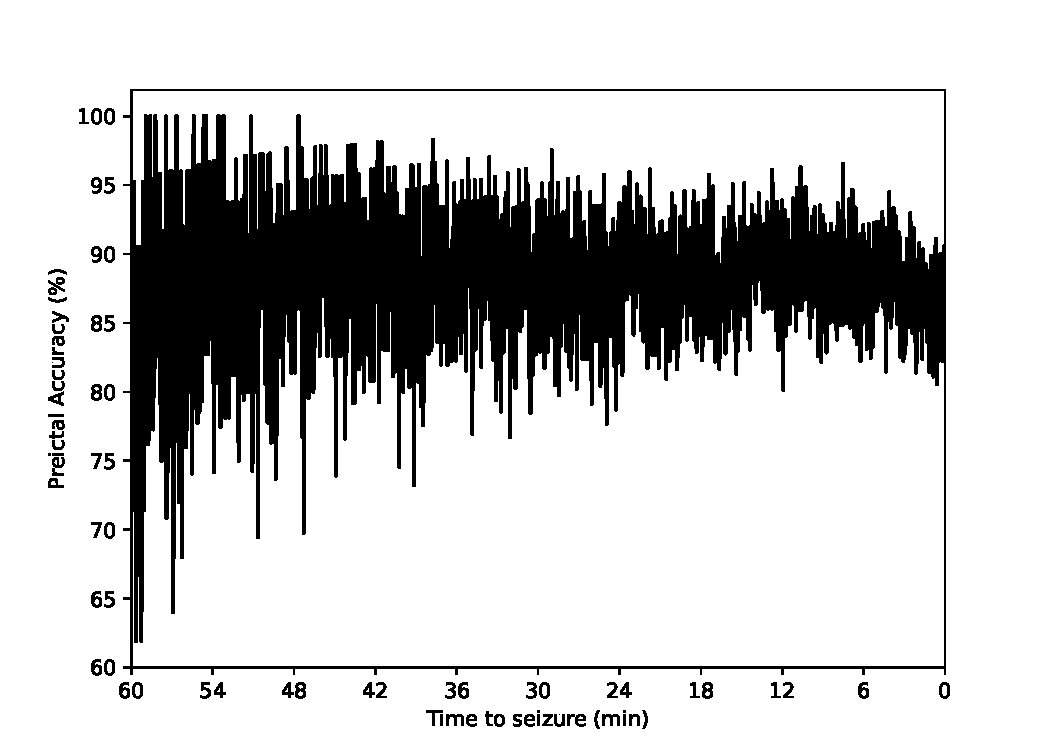
\includegraphics[scale=0.45]{figures/horizon_lookback_3600_raw.pdf}
	        \caption{60 minutes preictal horizon}
	        \label{fig:preictal-accuracy-raw-60min}
         \end{subfigure}
	\caption{Plots showing the non-smoothed prediction accuracy for preictal class depending on samples' proximity to seizure.}
	\label{fig:predictive-horizon-raw}
\end{figure}
\FloatBarrier
\subsection{Explainability}
We computed the explainability scores both for feature and edge importance to evaluate the influence of the preictal period extension on the scores. We also computed the same inter-period differences of feature importances as for the original 10-minute preictal lookback. The results are shown in Fig. \ref{fig:feature-explainability-20-mins} to \ref{fig:feature-explainability-60-mins}. It can be seen that across all horizons, connectivity changes are not visible. Similar things hold for feature importances, except the 30-minute and 60-minute lookback horizons. In these cases, we observe changes in the preictal predictions, especially for the 60-minute lookback. Overall, the score of all features decreases, and the most relevant features change. Katz FD gains importance relative to the other features. We speculate that these changes can be related to the observed drops in predictive performance for the more distant samples, indicating that the network starts using different indicators of these activities. We leave the in-depth analysis for further research.

\begin{figure}[h]
	\centering
	\begin{subfigure}{0.45\linewidth}
		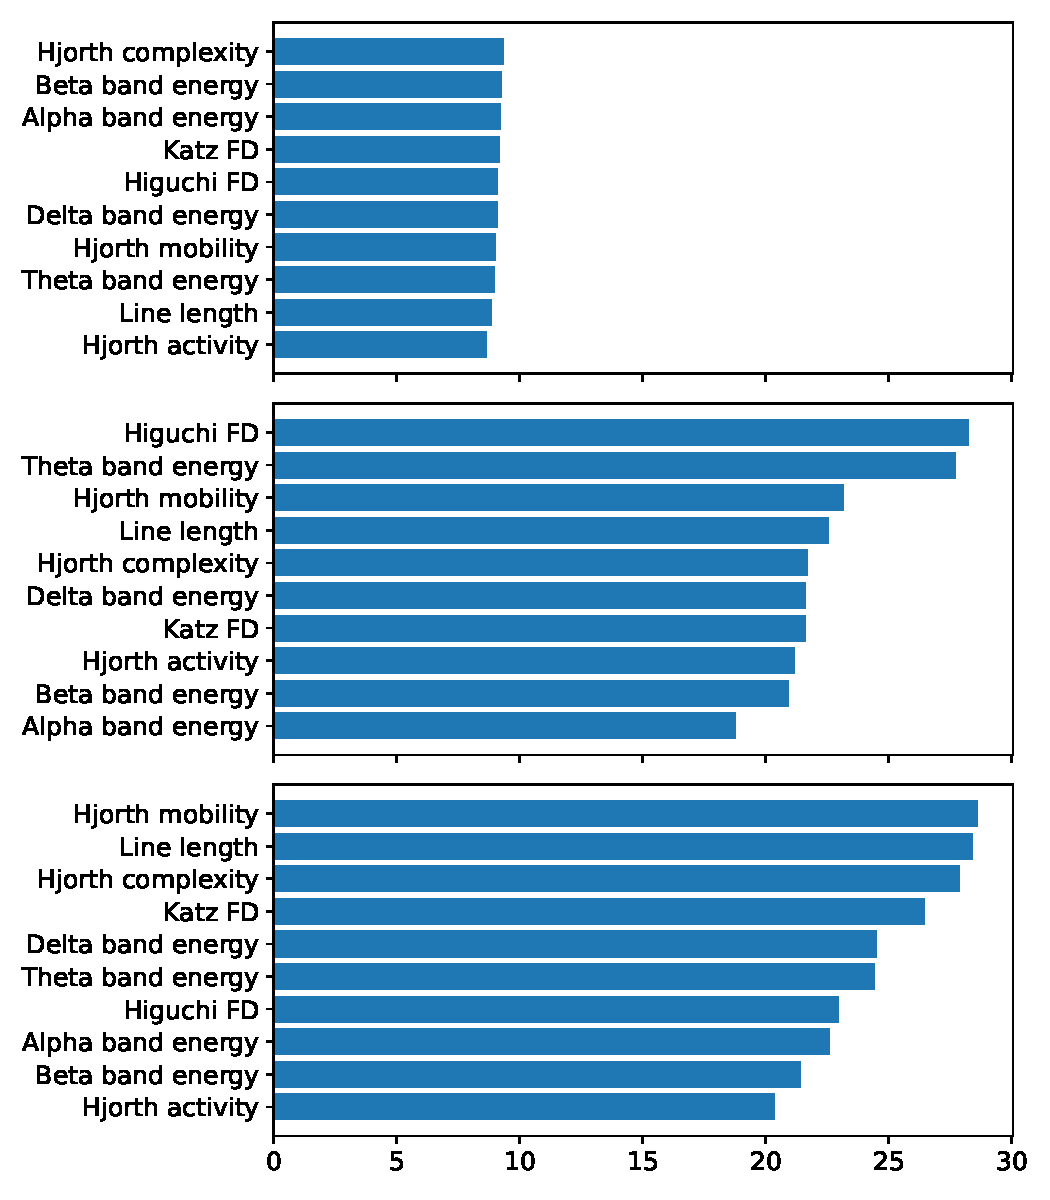
\includegraphics[scale=0.40]{figures/feature_importance_1200.pdf}
		\label{fig:feature-importance-relative-20mins}
	\end{subfigure}
	\begin{subfigure}{0.45\linewidth}
         \centering
		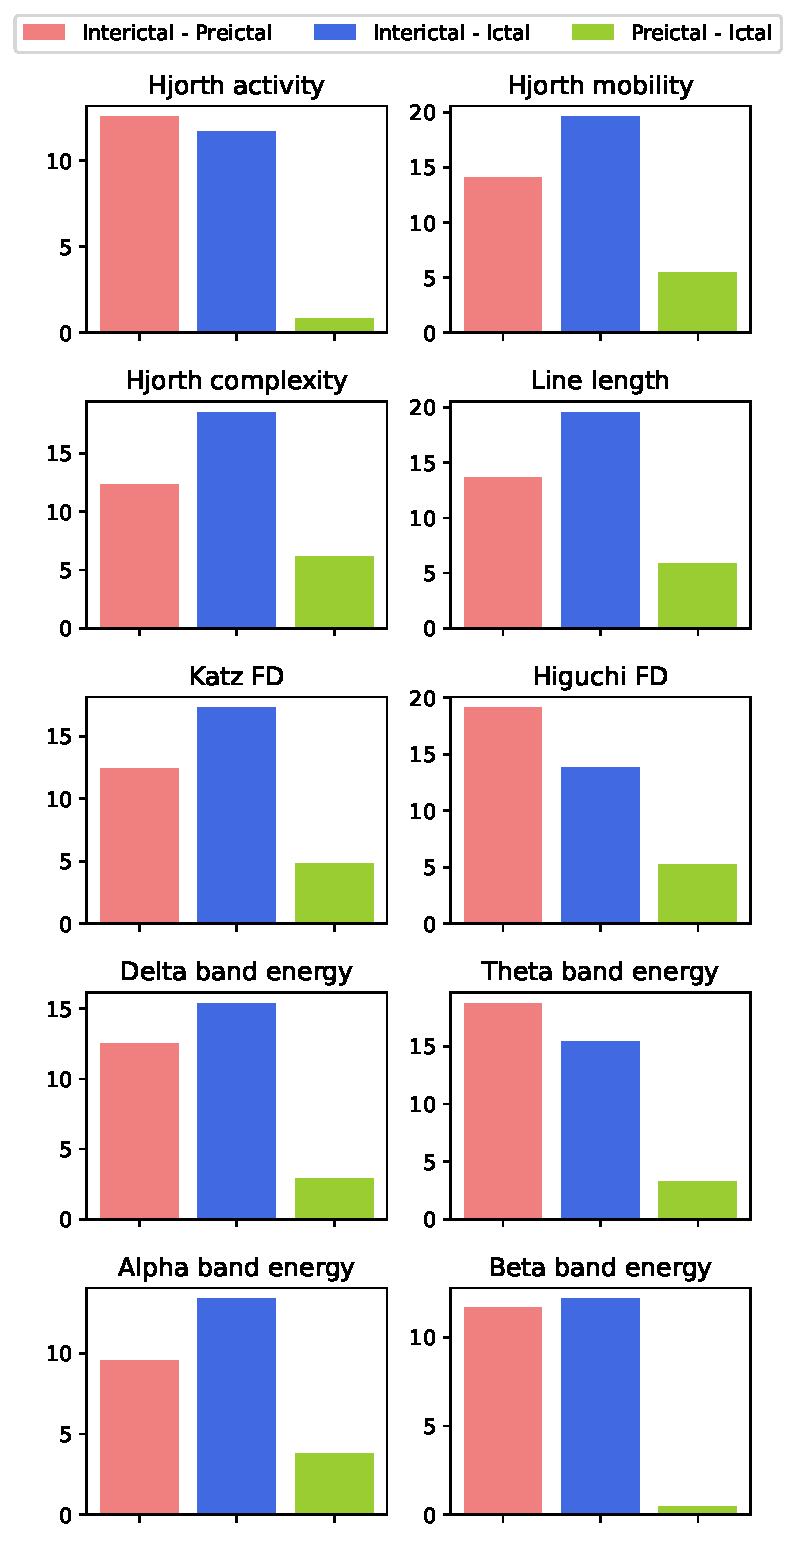
\includegraphics[scale=0.40]{figures/feature_importance_diffs_1200.pdf}
		\label{fig:feature-importance-diffs-20mins}
	\end{subfigure}
        \vfill
        \begin{subfigure}{1\linewidth}
        \centering
		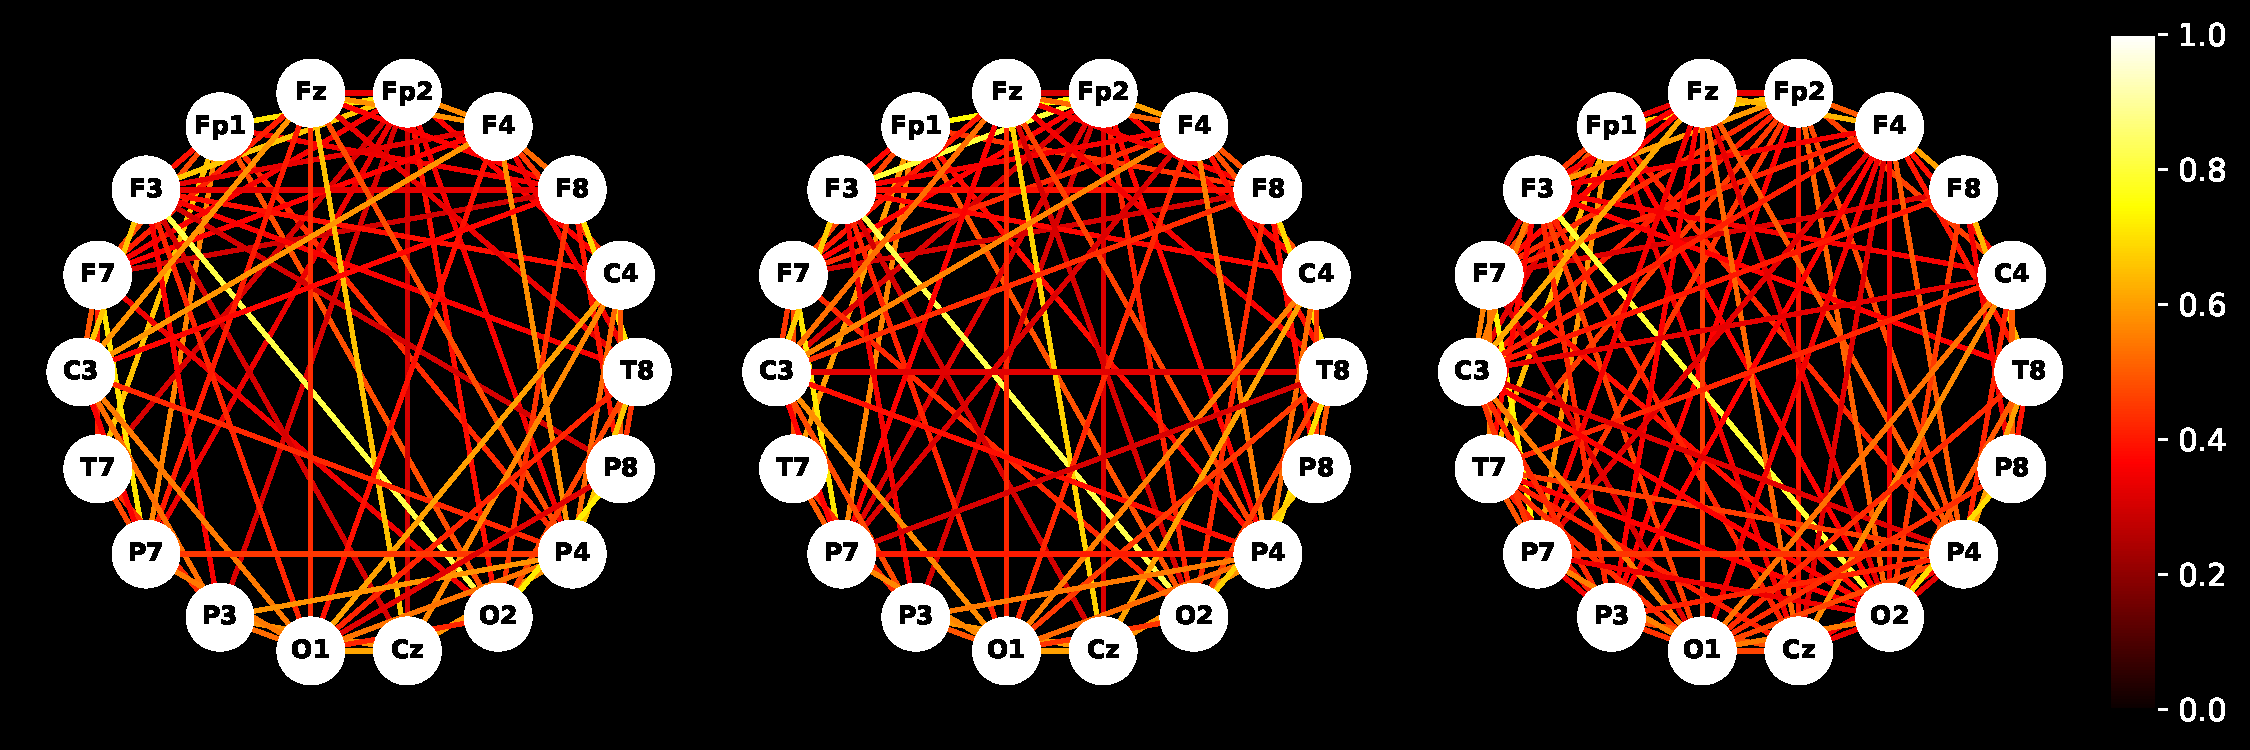
\includegraphics[scale=0.3]{figures/conncectivity_1200.pdf}
		\label{fig:connectivity-20mins}
	\end{subfigure}
	\caption{Plots showing the analysis of feature importance for experiments with the interictal horizon of 20 minutes. Top right: average node feature importance scores obtained from predictions on every sample across all folds. Top: interictal class, middle: preictal class, bottom: ictal class. Top left: Differences in importance scores between predictions
for chosen classes. Bottom: Edge importance scores based on attention coefficients obtained from predictions on every sample across all folds for different preictal horizons. Edges with attention scores below 0.2 are not shown for clarity. Self-loops are not visualized. Left: interictal class; center: preictal class; right: ictal class.}
	\label{fig:feature-explainability-20-mins}
\end{figure}
\FloatBarrier
\begin{figure}[h]
	\centering
	\begin{subfigure}{0.45\linewidth}
		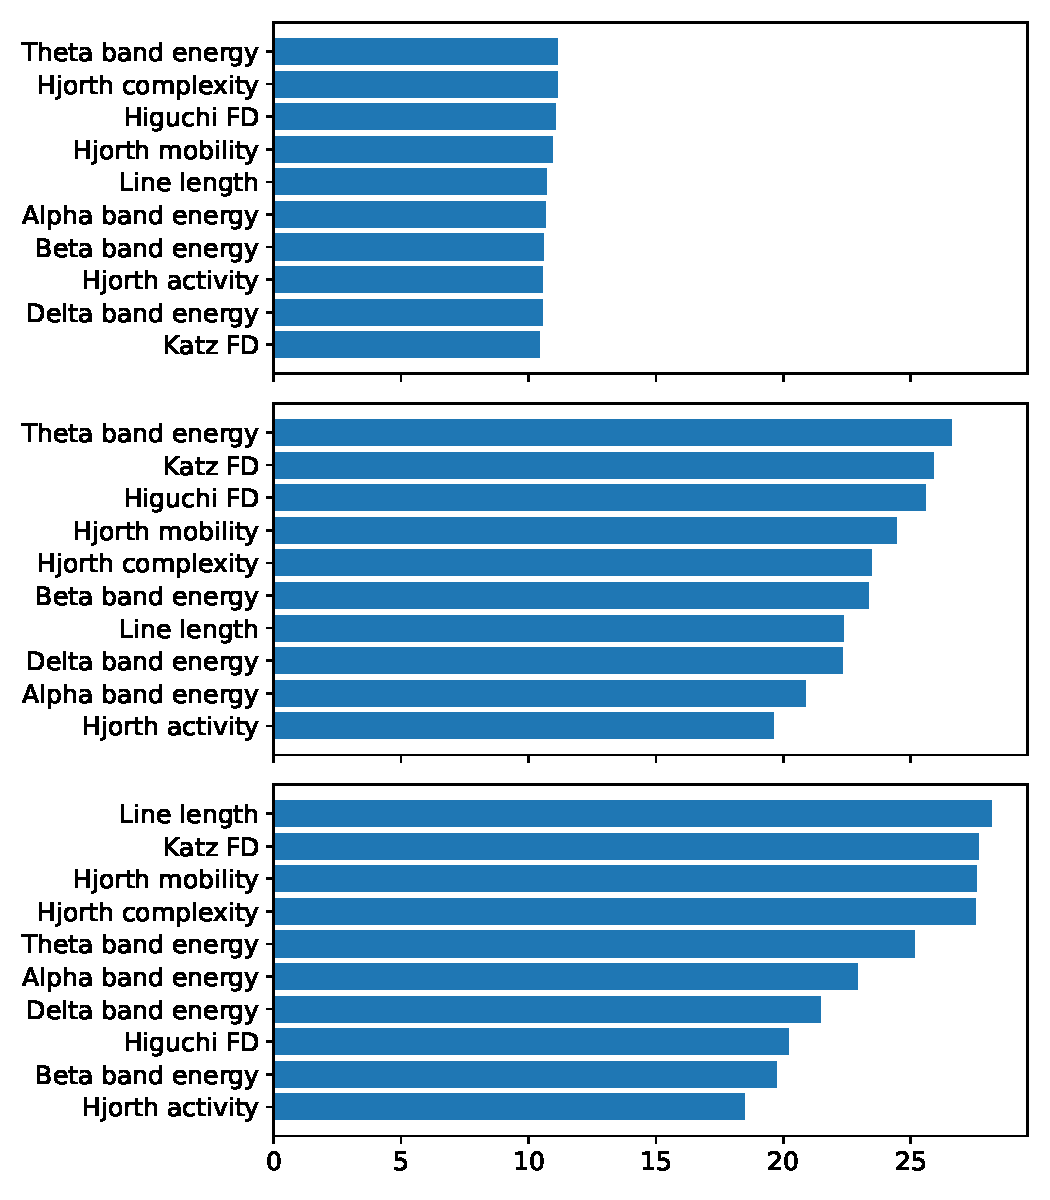
\includegraphics[scale=0.40]{figures/feature_importance_1800.pdf}
		\label{fig:feature-importance-relative-30mins}
	\end{subfigure}
	\begin{subfigure}{0.45\linewidth}
		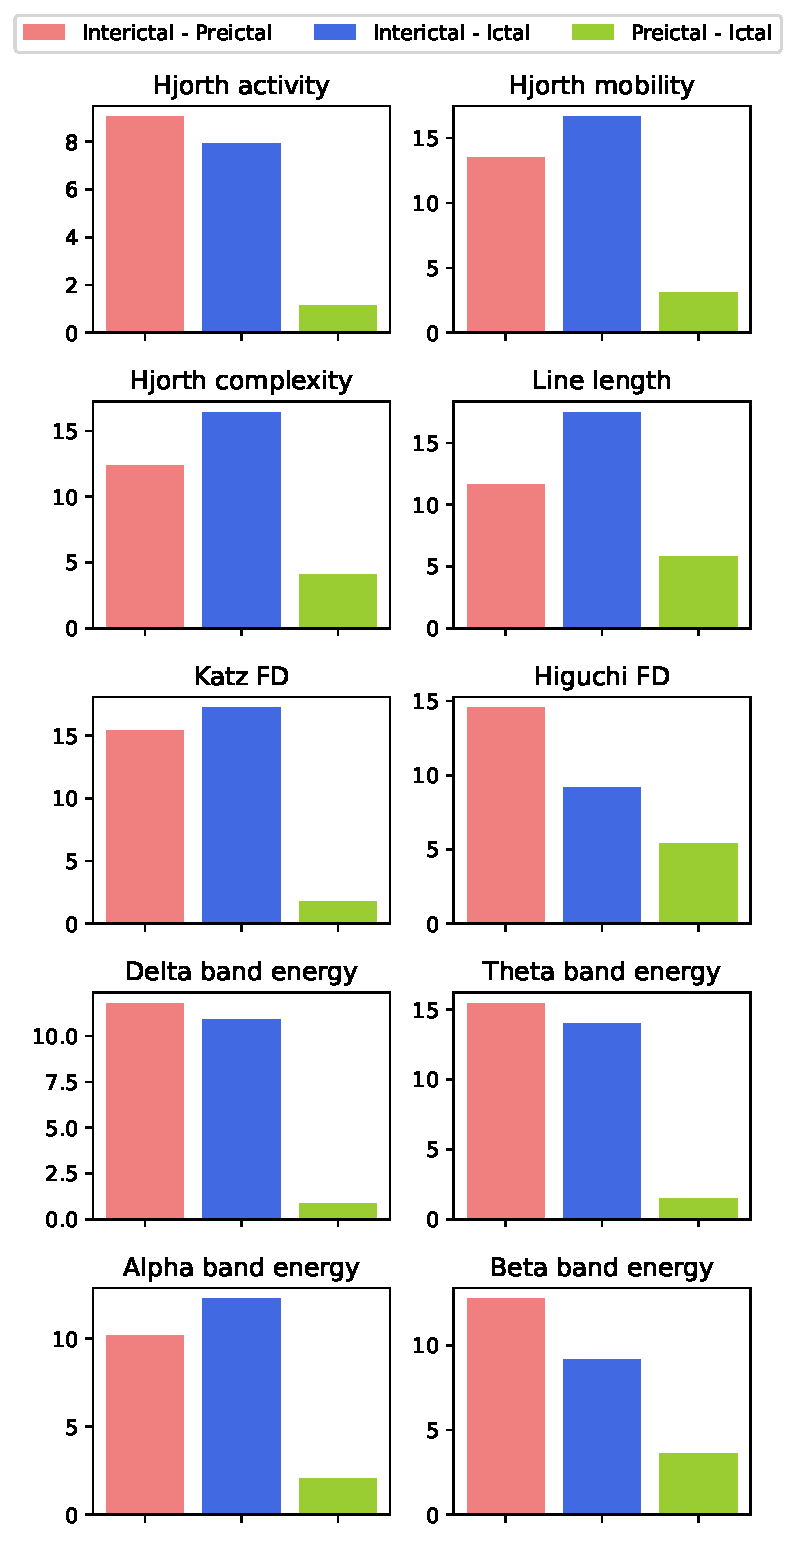
\includegraphics[scale=0.40]{figures/feature_importance_diffs_1800.pdf}
		\label{fig:feature-importance-diffs-30mins}
	\end{subfigure}
        \vfill
        \begin{subfigure}{1\linewidth}
        \centering
		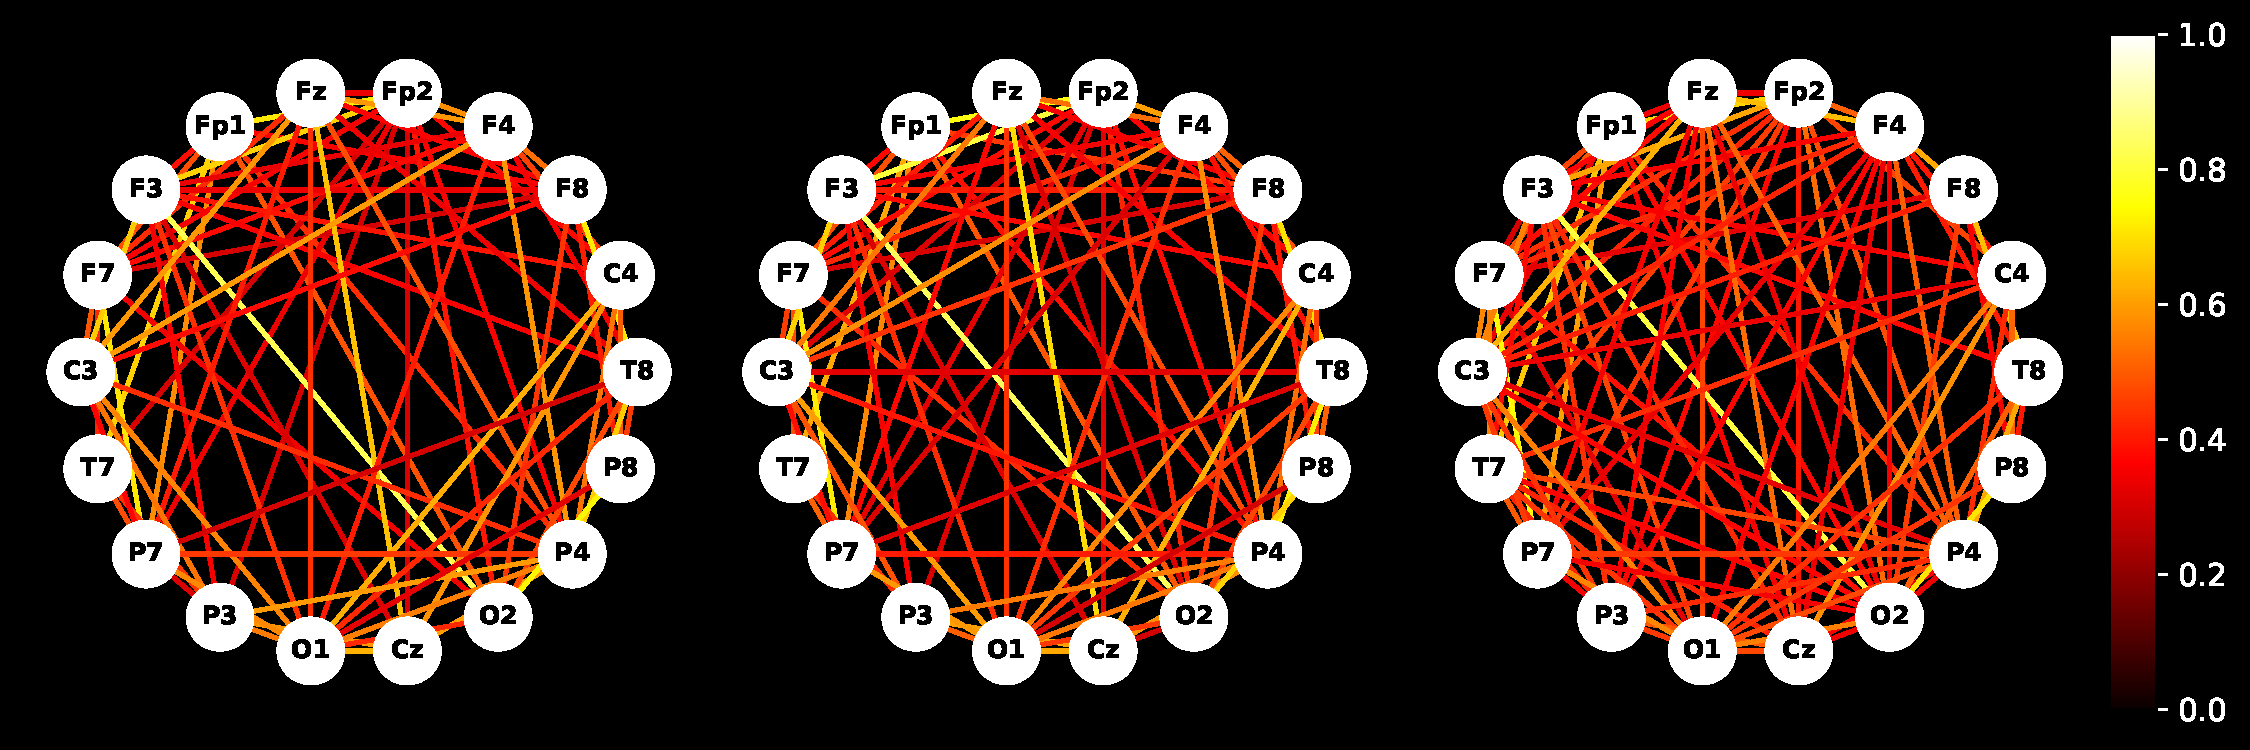
\includegraphics[scale=0.3]{figures/conncectivity_1800.pdf}
		\label{fig:connectivity-30mins}
	\end{subfigure}
	\caption{Plots showing the analysis of feature importance for experiments with the interictal horizon of 30 minutes. Top right: average node feature importance scores obtained from predictions on every sample across all folds. Top: interictal class, middle: preictal class, bottom: ictal class. Top left: Differences in importance scores between predictions
for chosen classes. Bottom: Edge importance scores based on attention coefficients obtained from predictions on every sample across all folds for different preictal horizons. Edges with attention scores below 0.2 are not shown for clarity. Self-loops are not visualized. Left: interictal class; center: preictal class; right: ictal class.}
	\label{fig:feature-explainability-30-mins}
\end{figure}
\FloatBarrier
\begin{figure}[h]
	\centering
	\begin{subfigure}{0.45\linewidth}
		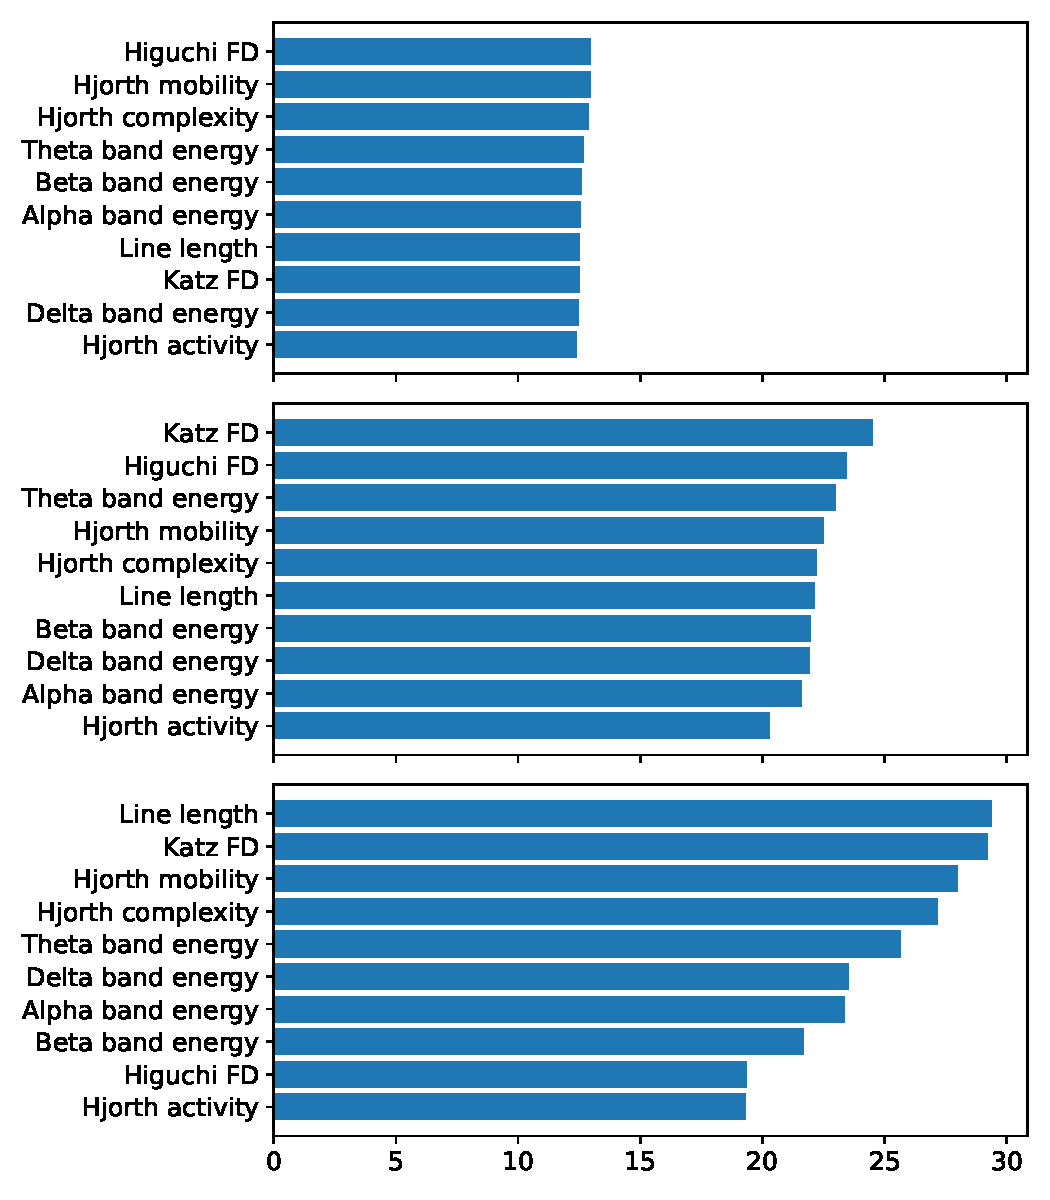
\includegraphics[scale=0.4]{figures/feature_importance_3600.pdf}
		\label{fig:feature-importance-relative-60mins}
	\end{subfigure}
	\begin{subfigure}{0.45\linewidth}
		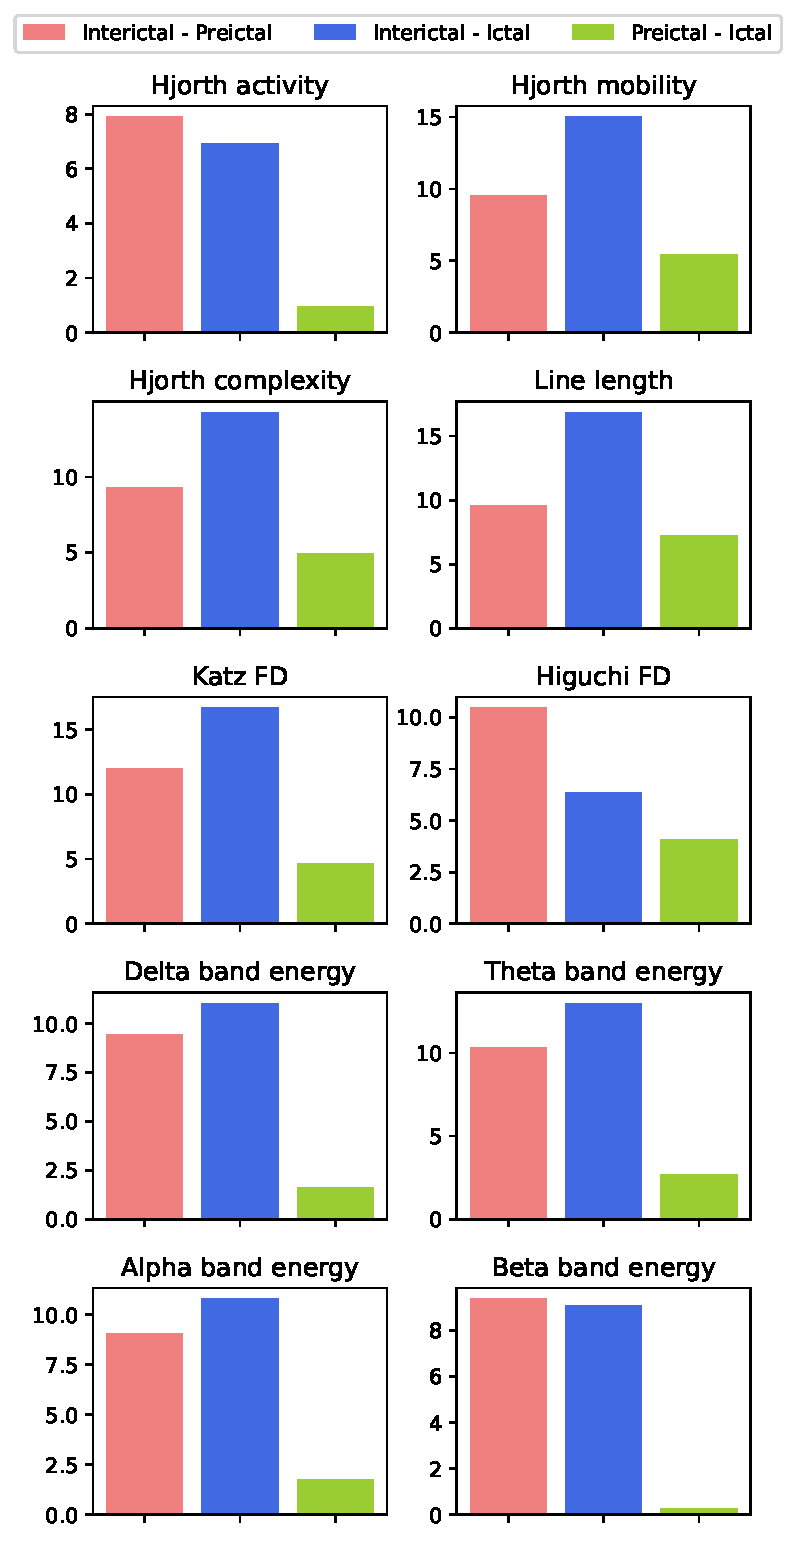
\includegraphics[scale=0.4]{figures/feature_importance_diffs_3600.pdf}
		\label{fig:feature-importance-diffs-60mins}
	\end{subfigure}
        \vfill
        \begin{subfigure}{1\linewidth}
        \centering
		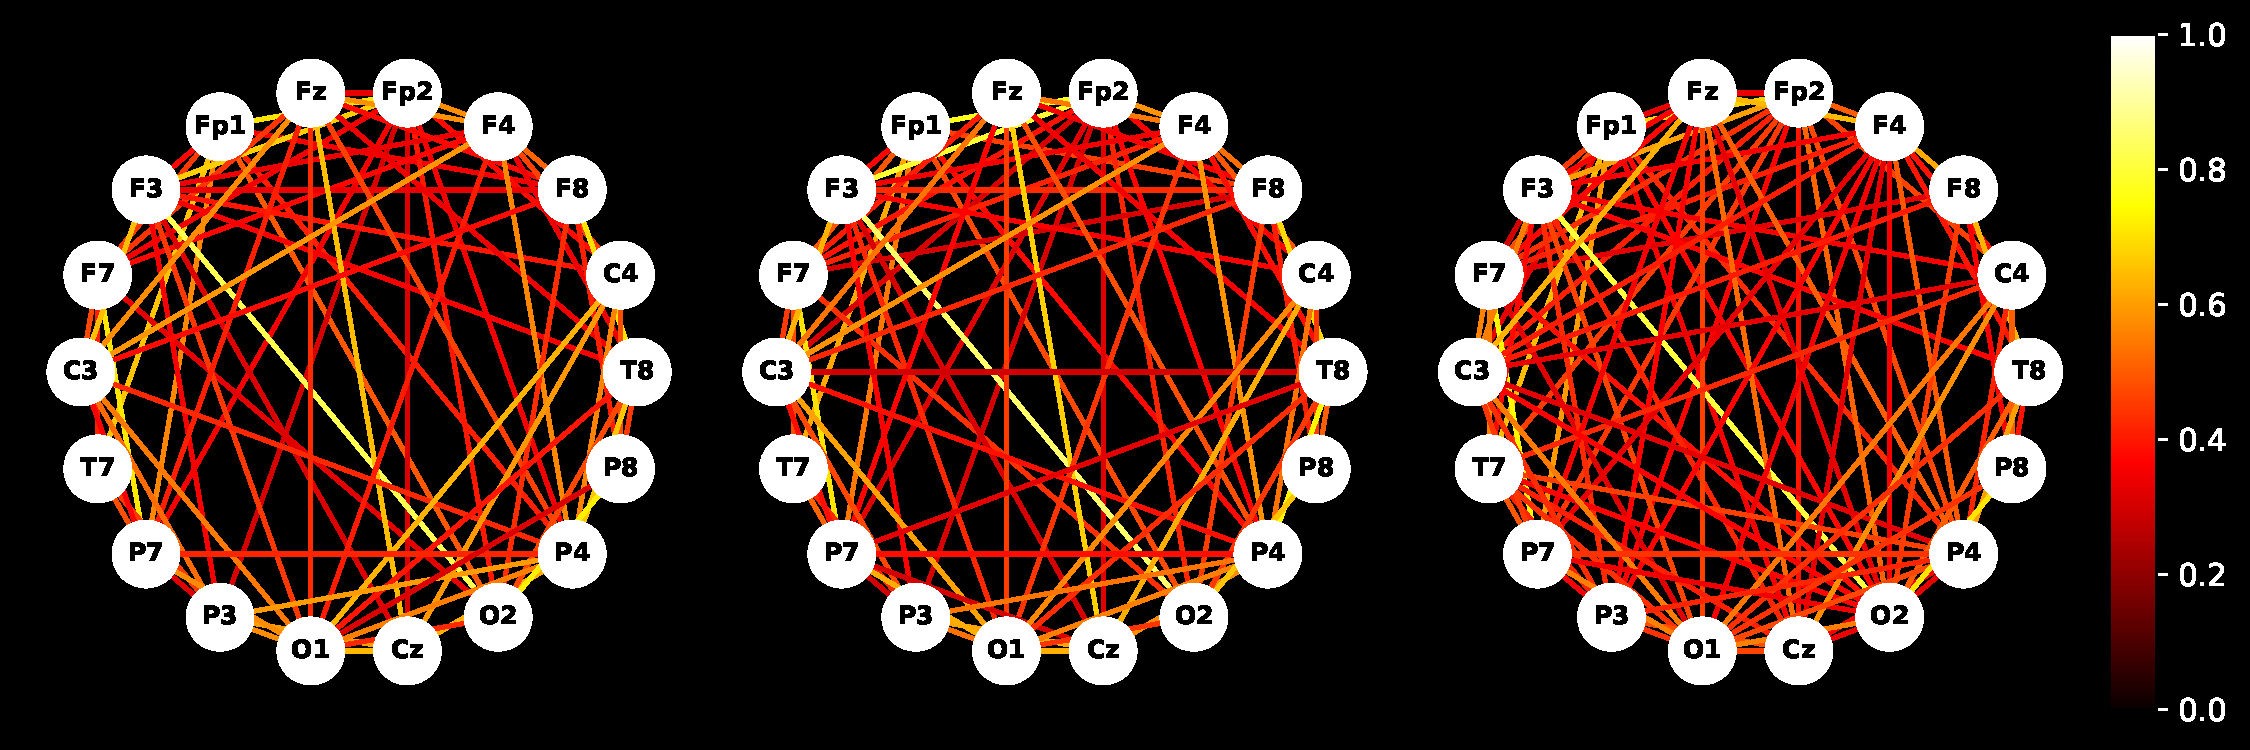
\includegraphics[scale=0.3]{figures/conncectivity_3600.pdf}
		\label{fig:connectivity-60mins}
	\end{subfigure}
 
	\caption{Plots showing the analysis of feature importance for experiments with the interictal horizon of 60 minutes. Top right: average node feature importance scores obtained from predictions on every sample across all folds. Top: interictal class, middle: preictal class, bottom: ictal class. Top left: Differences in importance scores between predictions
for chosen classes. Bottom: Edge importance scores based on attention coefficients obtained from predictions on every sample across all folds for different preictal horizons. Edges with attention scores below 0.2 are not shown for clarity. Self-loops are not visualized. Left: interictal class; center: preictal class; right: ictal class.}
	\label{fig:feature-explainability-60-mins}
\end{figure}
\FloatBarrier



\printcredits

\section*{Declaration of competing interests}
The authors declare no conflicts of interest.
\section*{Data availability}
The dataset is available at \url{https://physionet.org/content/chbmit/1.0.0/}. The code with the usage instructions is available at \url{https://github.com/szmazurek/sano_eeg}.
\section*{Acknowledgements}
This publication is supported by the European Union’s Horizon 2020 research and
innovation programme under grant agreement Sano No 857533.
This publication is supported by Sano project carried out within the International Research Agendas programme of the Foundation for Polish Science, co-financed by the European Union under the European Regional Development Fund. This research was supported in part by the PLGrid infrastructure on the Athena computer cluster.
%% Loading bibliography style file
\bibliographystyle{model1-num-names}
% \bibliographystyle{cas-model2-names}

% Loading bibliography database
\bibliography{cas-refs}


%\vskip3pt

\bio{figures/szymon.jpeg}
Szymon Mazurek holds a master's degree in computer science from AGH University of Cracow, where he is currently a PhD student in the same discipline. He is mainly interested in deep learning, especially graph-based, and the overall application of AI in medicine. For his PhD, he focuses on spiking neural networks and their performance enhancement with biologically plausible modulation. Currently, as a member Brain and More Lab, he works in the Sano Centre for Computational Medicine. He is also a research engineer at ACC Cyfronet AGH, where he is involved in using HPC for large-scale AI computations.
\endbio

\bio{figures/rosmary_elsvier.jpg}
Rosmary Blanco is a biotechnologist and a Neuroscience Ph.D. student at the Sano Centre for Computational Medicine. Her research focuses on investigating brain dynamics using diverse models, methods, and techniques, including EEG and fNIRS, to understand the large-scale network principles governing neuronal communication, cognition, and human behavior. She also integrates emerging technologies, utilizing wearable devices as cost-effective solutions for real-world neurophysiological investigations to support decision-making in the diagnostic process.
\endbio

\bio{figures/joan.png}
Joan Falc\'o Roget studied physics and biophysics at the University of Barcelona and at the Autonomous University of Madrid. He is a PhD Student at Sano Centre for Personalised Computational doing research in functional, diffusion, and effective connectivity in clinically oriented frameworks. He is also active in the field of theoretical neuroscience and has done research in normative models of animal behavior and in quantum computing solutions applied to computational neuroscience as well as medicine. He is currently employed as a teaching assitant at the AGH University of Cracow.
\endbio

\bio{figures/alex.jpeg}
Dr. Alessandro Crimi completed his studies in engineering at the University of Palermo,  obtained a PhD in machine learning applied for medical imaging from the University of Copenhagen,  and an MBA in healthcare management from the University of Basel.   
Alessandro worked as a post-doctoral researcher at the French Institute for Research in Computer Science (INRIA), the Technical School of Switzerland (ETH-Zurich), the Italian Institute for Technology (IIT), and the University Hospital of Zurich. In those institutes, he made significant contributions to the field of computational neuroscience. He taught for 8 years at the African Institute for Mathematical Science (AIMS) in Ghana and South Africa the course of machine learning in medicine, where he also supervised numerous MSc theses. Currently, he is a research group leader at Sano Centre for Computational Medicine and a professor at the AGH University of Cracow in Poland. Dr. Crimi is also currently involved in initiatives to promote entrepreneurship with women and individuals with immigrant backgrounds, as well as technology transfer projects for young scientists.
\endbio

\end{document}

